\chapter{Introduction}

The growing number of applications of computer programs in the past few decades brings
the~need for their greater safety and security.
But it is not an easy task to guarantee that a software has the specified properties.
The~programs often go through many states during the computations
and it could be very time and space consuming or even impossible to check whether no undesirable behavior
may appear in any of the program runs.
One of the approaches to ensure the software quality is \emph{testing} (and dynamic analysis) which is based
on running the program in different contexts with different inputs
and matching a program behavior and the outputs with the expected ones.
This method can satisfy the most of the software quality requirements and often covers the most of the program behavior.
On the~other side, it is only possible to find the~errors using testing, not to prove their absence~\cite{dijkstra}.
Finding some of the errors during testing also does not imply the elimination of all of them.

The mentioned weakness of testing can be resolved by \emph{formal verification}.
Formal verification aims at using rigorous mathematical methods to check whether a given system meets a given specification \cite{fav:lecture}.
There are three main branches of formal verification.
The first one is \emph{model checking} which systematically explores the state space of a~system (e.g., a program) or its model to
prove that it satisfies the verified property.
The second one is \emph{static analysis} which is performed over a source code (or some modification of it) of a~system
without a need of its explicit execution and it rather explores a syntactic structure of the analysed program.
One of the important and very widely used approaches in static analysis is called \emph{abstract interpretation} where the analysis is performed by
applying abstract transformers corresponding to the original program semantics over an abstract domain.
Model checking and static analysis are overlapping in present.
Abstract interpretation is an example of technique that is consider
to be the static analysis technique but it also has some attributes of
the model checking techniques.
The last approach is \emph{theorem proving}.
It proves the program safety in the standard mathematical way\,---\,starting
from axioms and using inference rules to verify properties of the given system.
Theorem proving can be partially automated.

This work deals with a specific branch of static analysis called \emph{shape analysis} which focuses on verification of programs manipulating
complex dynamic data structures (such as different kinds of lists and trees), typically allocated on the heap.
Checked properties are for example absence of invalid pointer dereference,
whether no invalid pointer is freed (no invalid free) or
whether all allocated memory is freed during the program execution (no memory leaks).
There are different approaches to shape analysis with different advantages.
The approaches based on \emph{separation logic} \cite{seplog,seplog07} provide great scalability.
On the~other hand, automata based approaches, particularly \emph{abstract regular tree model checking} (ARTMC) \cite{artmc}, are
superior in their flexibility and generality (but some state-of-the-art separation logic methods
have comparable generality \cite{biabduction}).
This work focuses on a verification procedure based on the concept of forest automata (FA) which
combines the benefits of the both mentioned approaches \cite{forester11}.

Forest automata have been introduced in \cite{forester11} and
they are an extension of finite tree automata (TA).
They are used as an abstract domain in a verification procedure which performs symbolic execution of the analyzed program.
A~prototype of this verification procedure has been implemented as the \emph{Forester} tool	\cite{www:forester}.
Forester verifies programs written in C and it can detect safety violations such as invalid dereferences, invalid frees,
memory leaks, and also reachability of an error line.
It is capable of verifying non-trivial data structures such as skip-lists of the~second and the~third level.
However, the current implementation is far from perfect.
For instance, Forester currently does not fully support the complete syntax of C and %TODO
it also does not check whether a found error is real or spurious.
A~general goal of this work is to improve Forester in the areas described further.

One of the problems of Forester is low modularity and maintainability of the code.
The first goal of this thesis is to improve it by changing the~underlying implementation
of finite tree automata in Forester to \vata\,---\,a state-of-the-art library for manipulation with TA \cite{libvata}.
%This should bring better maintainability and modularity than having
%a special TA library implementation within Forester as it is now.
The VATA library implements very efficiently the most of state-of-the-art algorithms for TA
and it is better to implement the algorithms efficiently with implementation optimizations
only at the one place (in VATA) than putting effort to optimizing the implementation
of the same algorithms in Forester again.
This improves the \emph{maintainability} of Forester.
Having the special encapsulated module for tree automata with a clear interface
brings also the \emph{modularity} by decreasing the dependencies on the internals of
the tree automata module.
%The code with implementation optimization is also not easy maintainable in long term.
%So it is again better to put this effort only once in the VATA library.
But it is needed to refactor some parts of Forester code before the changes.
Then it would be possible to create an interface between Forester and VATA.

Another weakness of Forester is lack of the analysis of detected errors.
Since Forester uses abstraction to deal with unboudness of dynamic data structures
a found error can be spurious what is caused by overapproximating
the set of reachable heap configurations by abstraction.
When this happens then the analysis of the detected error can determine
whether the error is a real or not.
The results of the counterexample analysis can be also used for refinement of abstraction.
Then the analysis can be restarted with the refined abstraction.
This gradual refinement of abstraction is based on \emph{counterexample-guided abstraction refinement} (CEGAR) \cite{cegar}.
%The verification procedure cannot verify correct programs with detected spurious error without this refinement.
%It can also detect a spurious error instead of the real one because the verification procedure ends after the
%first error detection without the analysis of the found error.
The second goal of this thesis is to design and implement the analysis of the counterexamples
and a refinement of abstraction (when a spurious error is found).
The method for analysing counterexamples is in this case \emph{backward run}
and its results will be further used for refinement of \emph{predicate abstraction}.
Forester does not currently use the mentioned predicate abstraction but \emph{height abstraction}
because predicate abstraction needs backward run for creating the new predicates for refinement.
Height abstraction is less precise and less flexible compared to predicate abstraction.
Predicate abstraction enables the analysis of even more complex data structures like red-black trees.

The outline of this master thesis is as follows.
In Chapter \ref{ch:prel}, the preliminaries are given.
The verification procedure based on FA is covered in Chapter \ref{ch:fav}.
Chapter \ref{ch:tools} provides description of \vata\ and Forester
and Chapter \ref{ch:fova} describes an implementation of the version of Forester tool using \vata.
The design and the implementation of backward run and predicate abstraction
is given in Chapter \ref{ch:backward}.
Finally, Chapter \ref{ch:eval} contains an overview of experimental evaluation and 
Chapter \ref{ch:concl} summarizes this thesis.

\chapter{Preliminaries}
\label{ch:prel}

This chapter provides the theoretical foundations for this thesis.
First, graphs, trees and forests are defined along the automata accepting them in Section~\ref{sec:graph}.
Then the previously defined concepts are further extended to hierarchical forests and automata in Section \ref{sec:fah}.
This section follows the definitions and the structure used in \cite{techrep}.

\section{Graphs, Trees and Forests}
\label{sec:graph}

Assume a alphabet $\Sigma$ and a word $w = a_1 \cdots a_n$, we denote the $i$-th symbol of $w$ from $\Sigma$ as $a_i$.
We denote $dom(f)$ the~domain of a total mapping $\funcdecl{f}{A}{B}$ and its range is denoted by $rng(f)$.

\subsection{Graphs and Trees}
\label{subsec:graph}
A \emph{ranked alphabet} is a finite set of symbols $\Sigma$ and a related mapping $\funcdecl{\#}{\Sigma}{\mathbb{N}}$
assigning to a symbol its rank.
A (directed, ordered, labelled) \emph{graph} is a total map $\funcdecl{g}{V}{\Sigma \times V^{*}}$ where $V$ is a finite set of nodes.
The items of the set $\Sigma$ are in context of the graphs called \emph{labels}.
The map $g$ maps each node $v\in V$ to:
\begin{enumerate}
	\item a label $\alpha \in \Sigma$ that we denote by $l_g(v)$.
	\item a sequence of \emph{successors} $(v_1 \cdots v_n) \in V^n$ for $n \in \mathbb{N}$.
		We denote successors by $S_g(v)$ and $v_i$ is denoted by $S^i_g(v)$.
\end{enumerate}
Symbol $l_g(v)$ is such that $\#(l_g(v)) = |S_g(v)|$.
We will omit the subscript $g$ when no ambiguity may arise possible.

A \emph{leaf} of $g$ is a node $v \in V$ such that $S_g(v) = \epsilon$.
An \emph{edge} of $g$ is a pair $v \mapsto (a, v_1 \cdots v_n)$ where $v, v_1, \ldots, v_n \in V$,
$a \in \Sigma$ such that $g(v) = (a, v_1 \cdots v_n)$.
The \emph{in-degree} of a node $v' \in V$ in the graph $g$ is the sum of
its occurrences in the tuples $t \in V^{*}$ get by $g(v)$ for all $v \in V$.
We denote the in-degree of a node $v \in V$ by $idg_g(v)$ and again
we omit the subscript $g$ whenever it is possible.
More formally, in-degree is defined as
$idg(v') = |\{(v \mapsto (a, v_1 \cdots v_n),i)) \,|\, v \mapsto (a, v_1 \cdots v_n)
\text{ is an edge such that } i \in \{1,\ldots,n\}: v' = v_i\}|$.
The \emph{joins} of $g$ are nodes $v \in V$ such that $idg(v') > 1$.

A \emph{path} from $v\in V$ to $v' \in V$ is a sequence $p=v_0, i_1, v_1, \ldots, i_n, v_n$ where $v=v_0, v' = v_n$
and $\forall j \in \{1,\ldots,n\}: v_j = S^{i_j}(v_{j-1})$ (informally, $v_j$ is the $i_j$-th successor of $v_{j-1}$).
The empty path has $n=0$.
The path $p$ has \emph{length} $n$ denoted by $length(p) = n$.
The path $p=u_0,i_1,u_1,\ldots,i_n,u_n$ is acyclic if $\forall u_i,u_j \in p: i \neq j \Rightarrow u_i \neq u_j$.
The \emph{cost} of the acyclic path $p$ is the sequence $i_1, \ldots, i_n$.
The path $p$ is \emph{cheaper} than path $p'$ iff the cost of $p$ is lexicographically smaller than that of $p'$. 
A node $u \in V$ is \emph{reachable} from a node $v \in V$ iff there exists a path from $v$ to $u$ or $u=v$.
A node $u \in V$ is a \emph{root} of the graph $g$ iff all nodes $v \in V$ are reachable from $u$.
We use the term $root$ also for a mapping $\funcdecl{root}{g}{V}$ which maps a graph to its root.
A graph with the root is called \emph{rooted}.

A \emph{tree} $t$ is a graph which is either empty, or it has exactly one root and $\forall v \in V: idg(v) \leq 1$ (informally,
each node is a successor of at most one of the other nodes).

\bexmp
We illustrate some terms related to the graphs and trees.
Consider a graph $t$ in Figure \ref{fig:graph_tree}
with $V=\{v_1,v_2,v_3,v_4,v_5\}$ and
the alphabet $\Sigma = \{a,b\}$ with a ranking function $\#$ such that $\#(a) = 2$ and $\#(b) = 0$.
Then the graph $t$ is the mapping $\{t(v_1) \mapsto (a, (v_2,v_3))$, $t(v_2) \mapsto (b, ())$,
$t(v_3) \mapsto (a, (v_4, v_5))$, $t(v_4) \mapsto (b, ())$, $t(v_5) \mapsto (b, ())\}$.
The node $v_2, v_4, v_5$ are leaves.
An example of an edge is $v_1 \mapsto (a,(v_2,v_3))$.
A path is for instance the sequence $v_1, 2, v_3, 2, v_5$
what is the path from $v_1$ to $v_5$.
Thus the node $v_5$ is reachable from the node $v_1$.
Since all nodes are reachable from $v_1$ then $v_1$ is a root of $t$.
No node has more then one incoming edge, hence $t$ is a tree.

	\begin{figure}[bth]
		\begin{center}
			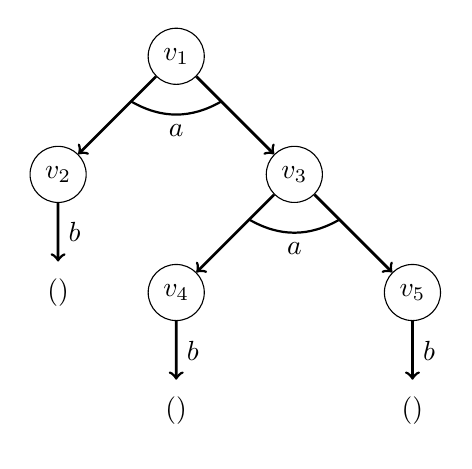
\begin{tikzpicture}[
  scale=0.8,
  node distance = 1.5cm,
  tnode/.style={circle, text centered, draw=black},
  lnode/.style={circle, text centered},
  arw/.style={->, line width=1pt},
  symline/.style={-, line width=0.8pt}
  ]

\node [tnode] (v1) {$v_1$};
\node [tnode, left of=v1, below of=v1] (v2) {$v_2$};
\node [left of=v1, below of=v1, above of=v2, right of=v2, yshift=1cm, xshift=0.8cm] (v1v2) {};
\node [tnode, right of=v1, below of=v1] (v3) {$v_3$};
\node [left of=v1, below of=v1, above of=v3, right of=v3, yshift=1cm, xshift=-0.8cm] (v1v3) {};
\node [lnode, below of=v2] (v02) {$()$};

\node [tnode, below of=v3, left of=v3] (v4) {$v_4$};
\node [left of=v3, below of=v3, above of=v4, right of=v4, yshift=1cm, xshift=0.8cm] (v3v4) {};
\node [tnode, below of=v3, right of=v3] (v5) {$v_5$};
\node [left of=v3, below of=v3, above of=v5, right of=v5, yshift=1cm, xshift=-0.8cm] (v3v5) {};
\node [lnode, below of=v4] (v04) {$()$};
\node [lnode, below of=v5] (v05) {$()$};

\draw [arw] (v1) -- (v2);
\draw [arw] (v1) -- (v3);
\draw [arw] (v2) -- node [midway, right] {$b$} (v02);
\draw [arw] (v3) -- (v4);
\draw [arw] (v3) -- (v5);
\draw [arw] (v4) -- node [midway, right] {$b$} (v04);
\draw [arw] (v5) -- node [midway, right] {$b$} (v05);

\draw [symline] (v1v2) edge [bend right] node [midway, below] {$a$} (v1v3);
\draw [symline] (v3v4) edge [bend right] node [midway, below] {$a$} (v3v5);

\end{tikzpicture}

		\end{center}
		\caption{A graph $t$ that has attributes of a tree.}
		\label{fig:graph_tree}
	\end{figure}
	\label{ex:graph}
\eexmp

\subsection{Forests}
\label{subsec:forests}

Without the loss of generality suppose that $\Sigma \cap \mathbb{N} = \emptyset$.
A $\Sigma$-labelled \emph{forest} is a sequence of trees $t_1 \cdots t_n$ over ($\Sigma \cup \{1,\ldots,n\}$)
where $\forall i \in \{1,\ldots,n\}: \#i = 0$.
We suppose that the sets of nodes of the trees $t_1, \ldots, t_n$ are disjoint.
\emph{Root references} are leaves labelled by $i \in \mathbb{N}$.
The forest $t_1 \cdots t_n$ represents the graph $\fagr$ that arises
by interconnecting roots by the related root reference.
For instance, a root reference $2$ in $t_1$ would be replaced by the root node of $t_2$.
Let us formalize the idea of the construction of $\fagr$.
The graph $\fagr$ contains an edge $v \mapsto (a,v_1 \cdots v_m)$ iff $\exists i \in \{1, \ldots, n\}:\ \exists(v \mapsto (a, v_1' \cdots v_m')) \in edges(t_i):
\ \forall j \in \{1,\ldots,m\}: v_j = h(v_j')$ where $edges(t_i)$ is the set of all edges of the tree $t_i$ and
\[ h(v_j') = \left\{
  \begin{array}{l l}
  root(t_k) & \quad \text{if $v_j'$ is a root reference with $l(v_j') = k$}\\
  v_j'   & \quad \text{otherwise.}
  \end{array} \right.\]

\pagebreak
\bexmp
We illustrate the notion of forest.
Consider a forest $f$ in Figure \ref{fig:forest}.
It consists of three trees: $t_1$ with the root $u_1$,
$t_2$ with the root $v_1$, and $t_3$ with the root $w_1$.
The alphabet $\Sigma$ of the trees is the same as in Example \ref{ex:graph} but $f$
is defined over $\Sigma \cup \{\overline{2}, \overline{3}\}$
where $\overline{2}, \overline{3}$ denotes the root references
to the roots $u_5$ and $v_3$ of the second and the third tree.

We can obtain a graph $\otimes t_1,t_2,t_3$ shown in Figure \ref{fig:forest_grap} from $t_1, t_2, t_3$.
The edges labelled by root references are replaced by the edges leading to the roots
of the referenced trees.
	\begin{figure}[bth]
	\begin{center}
		\scalebox{1}
		{
			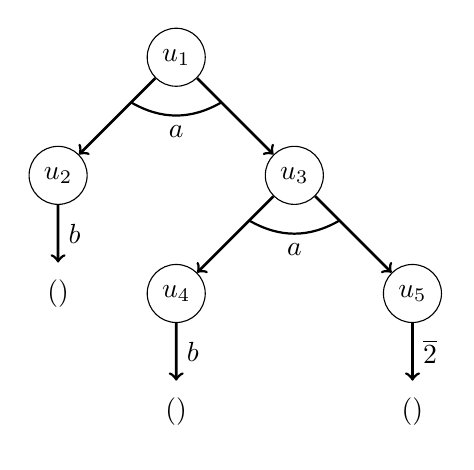
\begin{tikzpicture}[
  scale=0.8,
  node distance = 1.5cm,
  tnode/.style={circle, text centered, draw=black},
  lnode/.style={circle, text centered},
  arw/.style={->, line width=1pt},
  symline/.style={-, line width=0.8pt}
  ]

\node [tnode] (u1) {$u_1$};
\node [tnode, left of=u1, below of=u1] (u2) {$u_2$};
\node [left of=u1, below of=u1, above of=u2, right of=u2, yshift=1cm, xshift=0.8cm] (u1u2) {};
\node [tnode, right of=u1, below of=u1] (u3) {$u_3$};
\node [left of=u1, below of=u1, above of=u3, right of=u3, yshift=1cm, xshift=-0.8cm] (u1u3) {};
\node [lnode, below of=u2] (u02) {$()$};

\node [tnode, below of=u3, left of=u3] (u4) {$u_4$};
\node [left of=u3, below of=u3, above of=u4, right of=u4, yshift=1cm, xshift=0.8cm] (u3u4) {};
\node [tnode, below of=u3, right of=u3] (u5) {$u_5$};
\node [left of=u3, below of=u3, above of=u5, right of=u5, yshift=1cm, xshift=-0.8cm] (u3u5) {};
\node [lnode, below of=u4] (u04) {$()$};
\node [lnode, below of=u5] (u05) {$()$};

\draw [arw] (u1) -- (u2);
\draw [arw] (u1) -- (u3);
\draw [arw] (u2) -- node [midway, right] {$b$} (u02);
\draw [arw] (u3) -- (u4);
\draw [arw] (u3) -- (u5);
\draw [arw] (u4) -- node [midway, right] {$b$} (u04);
\draw [arw] (u5) -- node [midway, right] {$\overline{2}$} (u05);

\draw [symline] (u1u2) edge [bend right] node [midway, below] {$a$} (u1u3);
\draw [symline] (u3u4) edge [bend right] node [midway, below] {$a$} (u3u5);

\end{tikzpicture}

			\hspace{0.55cm}
			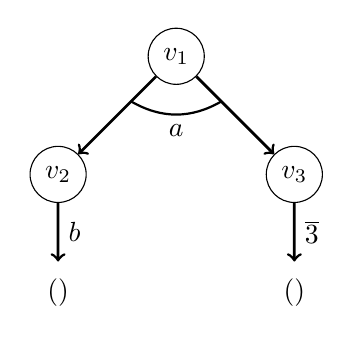
\begin{tikzpicture}[
  scale=0.8,
  node distance = 1.5cm,
  tnode/.style={circle, text centered, draw=black},
  lnode/.style={circle, text centered},
  arw/.style={->, line width=1pt},
  symline/.style={-, line width=0.8pt}
  ]

\node [tnode] (v1) {$v_1$};
\node [tnode, left of=v1, below of=v1] (v2) {$v_2$};
\node [left of=v1, below of=v1, above of=v2, right of=v2, yshift=1cm, xshift=0.8cm] (v1v2) {};
\node [tnode, right of=v1, below of=v1] (v3) {$v_3$};
\node [left of=v1, below of=v1, above of=v3, right of=v3, yshift=1cm, xshift=-0.8cm] (v1v3) {};
\node [lnode, below of=v2] (v02) {$()$};
\node [lnode, below of=v3] (v03) {$()$};

\draw [arw] (v1) -- (v2);
\draw [arw] (v1) -- (v3);
\draw [arw] (v2) -- node [midway, right] {$b$} (v02);
\draw [arw] (v3) -- node [midway, right] {$\overline{3}$} (v03);

\draw [symline] (v1v2) edge [bend right] node [midway, below] {$a$} (v1v3);

\end{tikzpicture}

			\hspace{0.55cm}
			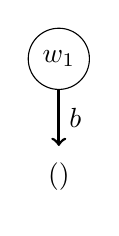
\begin{tikzpicture}[
  scale=0.8,
  node distance = 1.5cm,
  tnode/.style={circle, text centered, draw=black},
  lnode/.style={circle, text centered},
  arw/.style={->, line width=1pt},
  symline/.style={-, line width=0.8pt}
  ]

\node [tnode] (w1) {$w_1$};
\node [lnode, below of=w1] (w01) {$()$};

\draw [arw] (w1) -- node [midway, right] {$b$} (w01);

\end{tikzpicture}

		}
		\caption{A forest $f$ consisting 3 trees $t_1, t_2, t_3$ with roots $u_1, v_1, w_1$.}
	  \label{fig:forest}
	\end{center}
	\end{figure}

	\begin{figure}[bth]
	\begin{center}
		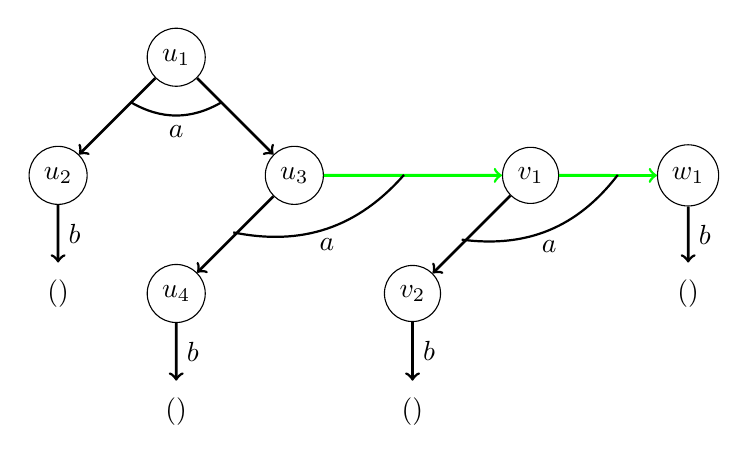
\begin{tikzpicture}[
  scale=0.8,
  node distance = 1.5cm,
  tnode/.style={circle, text centered, draw=black},
  lnode/.style={circle, text centered},
  arw/.style={->, line width=1pt},
  symline/.style={-, line width=0.8pt}
  ]

% tree 1

\node [tnode] (u1) {$u_1$};
\node [tnode, left of=u1, below of=u1] (u2) {$u_2$};
\node [left of=u1, below of=u1, above of=u2, right of=u2, yshift=1cm, xshift=0.8cm] (u1u2) {};
\node [tnode, right of=u1, below of=u1] (u3) {$u_3$};
\node [left of=u1, below of=u1, above of=u3, right of=u3, yshift=1cm, xshift=-0.8cm] (u1u3) {};
\node [lnode, below of=u2] (u02) {$()$};

\node [tnode, below of=u3, left of=u3] (u4) {$u_4$};
\node [left of=u3, below of=u3, above of=u4, right of=u4, yshift=0.8cm, xshift=0.6cm] (u3u4) {};
\node [lnode, below of=u4] (u04) {$()$};

\node [right of=u3, left of=v1, right of=u1, below of=u1, xshift=1.5cm, yshift=0.13cm] (u3v1) {};

\draw [arw] (u1) -- (u2);
\draw [arw] (u1) -- (u3);
\draw [arw] (u2) -- node [midway, right] {$b$} (u02);
\draw [arw] (u3) -- (u4);
\draw [arw] (u4) -- node [midway, right] {$b$} (u04);

\draw [symline] (u1u2) edge [bend right] node [midway, below] {$a$} (u1u3);

% tree 2
\node [tnode, right of=u1, right of=u3] (v1) {$v_1$};
\node [tnode, left of=v1, below of=v1] (v2) {$v_2$};
\node [left of=v1, below of=v1, above of=v2, right of=v2, yshift=0.7cm, xshift=0.5cm] (v1v2) {};
\node [lnode, below of=v2] (v02) {$()$};

\draw [arw] (v1) -- (v2);
\draw [arw] (v2) -- node [midway, right] {$b$} (v02);

%tree 3
\node [tnode, right of=v1, xshift=0.5cm] (w1) {$w_1$};
\node [lnode, below of=w1] (w01) {$()$};
\node [right of=v1, left of=w1, yshift=0.13cm, xshift=-0.8cm] (v1v3) {};

\draw [arw] (w1) -- node [midway, right] {$b$} (w01);

%\draw [arw] (w1) -- node [midway, right] {$b$} (w01);

%connection

\draw [arw, color=green] (u3) -- (v1);
\draw [arw, color=green] (v1) -- (w1);

\draw [symline] (u3u4) edge [bend right] node [midway, below] {$a$} (u3v1);
\draw [symline] (v1v2) edge [bend right] node [midway, below] {$a$} (v1v3);

\end{tikzpicture}

		\caption{The graph $\otimes t_1,t_2,t_3$ obtained from the forest $f$ in Figure \ref{fig:forest}.
		The green edges are the ones that were added to the graph created from the forest $f$.}
	  \label{fig:forest_graph}
	\end{center}
	\end{figure}
\vspace{-0.5cm}
\eexmp

\subsection{Graphs and Forests with Ports}
\label{subsec:gfp}

We extend the notion of graphs and forests with \emph{input} and \emph{output} nodes which are marked by so-called \emph{ports}.
An \emph{input-output-graph} (io-graph) is a pair $(g,\phi)$ (for brevity denoted as $g_\phi$)
where $g$ is a graph and $\phi=(\phi_1 \cdots \phi_n) \in dom(g)^+$ is a sequence of ports, $\phi_1$
is an input port and $\phi_2 \cdots \phi_n$ is a sequence of output ports.
The ports are unique in $\phi$.
The graph $g_\phi$ is called \emph{accessible} if its root is the input port $\phi_1$.

The set of \emph{cut-points} $cps(g_\phi)$ of a graph $g_\phi$ consists of its ports
and joins.
Formally, $cps(g_\phi)=\{v \in V\,|\, v \in \phi \vee idg(v) > 1\}$.

An \emph{io-forest} is a pair $f=(t_1 \cdots t_n, \pi)$ such that $n \geq 1$ and $\pi \in \{1,\ldots,n\}^n$
is a sequence of port indices, where $\pi_1$ is an index of input port and $\pi_2 \ldots \pi_{|\pi|}$ is a sequence of
the indices of the output ports.
As in the case of ports, the indices are unique.
The io-graph $\otimes f$ is constructed from a forest $f$ such that
$\otimes f = (\otimes t_1 \cdots t_n,root(t_{\pi_{1}}),\ldots,root(t_{\pi_{n}}))$.
The ports of $\otimes f$ are the roots of the~trees indexed by the indices in $\pi$.
This means that a node of the graph pointed by $\pi_1$ is an input port of $\otimes f$.
The nodes (that were the roots of the trees) pointed by the output port indices in $\pi$ are the output ports of $\otimes f$.

\bexmp
Recall the graph $t$ from Figure \ref{fig:graph_tree}.
It can be extended to an io-graph $t_\phi$ by adding ports $\phi=(v_1,v_4,v_5)$.
The resulting io-graph $t_\phi$ has the input port $v_1$ and the output ports $v_2,v_3$.
Because $v_1$ is the root, the graph $t_\phi$ is accessible.
The cut-points of $t_\phi$ are $v_1, v_4, v_5$.

In Figure \ref{fig:forest}, we shown the forest $f$.
This forest could be extended to an io-forest $f_{io}=((t_1,t_2,t_3),\pi)$ 
by defining a sequence of the port indices $\pi$ which could be e.g., $(1,3)$.
Then the graph $\otimes f_{io}$ is a pair $(\otimes (t_1,t_2,t_3)$, $(u_1,w_1))$.
The graph $\otimes (t_1,t_2,t_3)$ is the same as in Figure~\ref{fig:forest_graph}.
The input port $u_1$ is indeed $root(t_1)$
and the output port $w_1$ because it is the root of the third tree in $f$
and the index of the output port is $3$.
\label{ex:iograph}
\eexmp

\subsection{Minimal and Canonical Forest}
\label{subsec:mcforest}

There are two properties of the forests, minimality and canonicity, that we will further use.
The properties make it possible to represent an io-forest in a unique way.
%That enables deterministic manipulating with io-forest.
An io-forest $f=(t_1 \cdots t_n, \phi)$ representing a graph $\otimes f$ is \emph{minimal}
iff the roots of the trees $t_1,\ldots,t_n$ correspond to the cut-points of $\otimes f$,
so there exists a bijection between $\{root(t_k)\,|\, t_k \in \{t_1, \ldots, t_n\} )\}$ and $cps(\otimes f)$.
The minimal io-forest is hence a unique representation of $\otimes f$ up-to to permutations of $t_1,\ldots,t_n$.

To be able to define truly canonicity representation of the forest $f$
we define an ordering $\preceq_p$, so called \emph{canonical ordering}, of the cut-points of $\otimes f$.
The canonical ordering ${\preceq_p} \subseteq {cps(\otimes f) \times cps(\otimes f)}$
is defined as follows: $c_1 \preceq_p c_2 \Leftrightarrow \text{the cost of the cheapest path from }
\phi_1$ (input port) to $c_1 \text{ is}$ $\emph{smaller}$ $\text{ than the cost of the smallest path from } \phi_1 \text{ to } c_2$.
The io-forest $f_c$ is \emph{canonical} iff it is minimal, the trees $t_1,\ldots, t_n$ are ordered by $\preceq_p$, and $\otimes f$ is accessible.
The canonical io-forest is then a unique representation of an accessible io-graph.
The canonical io-forest can be obtained by a depth-first traversal (DFT)\cite{taocp} of $\otimes f$.
To make DFT traversal deterministic and hence the ordering of the trees unique
we need to assume that there is an ordering $\leq_\Sigma$ over labels $\Sigma$ of $\otimes f$.
The DFT then uses a stack of nodes initialized with the input and output ports
ordered by $\preceq_p$ with the smallest node on the top of the stack.
The DFT is run over $\otimes f$.
It visits the successors of a node in the order given by $\leq_{\Sigma}$ and
the nodes in successors tuples are in their order in tuple.
We obtain canonical forest $f_c$ where trees are in the following order.
The first ones are trees corresponding to the ports of $f$ ordered by $\preceq_p$
and the rest of the trees is in the canonical ordering of the trees
which is defined by the order of the DFT traversal visit.


\subsection{Tree Automata}
\label{subsec:ta}

A (finite, non-deterministic, top-down) \emph{tree automaton} (TA) is a
quadruple $A = (Q, \Sigma, \Delta, R)$ where
\begin{itemize}
	\item $Q$ is a finite set of \emph{states},
	\item $\Sigma$ is a ranked alphabet,
	\item $\Delta$ is a set of \emph{transition rules} where transitions have a form $(q,a,q_1 \cdots q_n)$ where $q,q_1,\ldots,q_n \in Q$, $a \in \Sigma$, $n \geq 0$ and $\#a = n$.
		Alternatively, we write $q \xrightarrow{a} (q_1 \cdots q_n)$ to denote that $(q,a,q_1 \cdots q_n) \in \Delta$.
		The rule is called \emph{leaf rule} when $n=0$,
	\item $R \subseteq Q$ is a set of \emph{root states}.
\end{itemize}

We can symmetrically define bottom-up tree automata as a quadruple $B = (Q, \Sigma, \Delta, F)$ where
\begin{itemize}
	\item $Q$ is a finite set of states,
	\item $\Sigma$ is a ranked alphabet,
	\item $\Delta$ is a set of transition rules where transition has a form $(q_1 \cdots q_n,a,q)$ where \linebreak $q,$$q_1,\ldots,q_n$ $\in Q$, $a \in \Sigma$, $n \geq 0$ and $\#a = n$.
		We can again write $(q_1 \cdots q_n) \xrightarrow{a} q$ to denote a $(q_1 \cdots q_n,a,q) \in \Delta$.
		For $n=0$ we call the rule \emph{leaf rule},
	\item $F \subseteq Q$ is a set of \emph{final states}.
\end{itemize}

We further consider top-down tree automata unless stated otherwise.

Their semantics of TA is defined following as follows.
A \emph{run} of $A$ over a tree $t$ is mapping $\funcdecl{\rho}{dom(t)}{Q}$ such that
$\forall v \in dom(t)\ \exists q \xrightarrow{a} (q_1 \cdots q_n) \in \Delta:  q=\rho(v) \wedge  \forall i \in \{1, \ldots, |S(v)|\}: q_i=\rho(S(v)_i)$.
We use $t \Rightarrow_{\rho} q$ to denote that $\rho$ is a run of $A$
over a tree $t$ s.t. $\rho(root(t)) = q$ and we use $t \Rightarrow q$ to denote that
exists $t \Rightarrow_{\rho} q$. % there exists run $\rho$ over $t$ to $q$.
The \emph{language} of a state $q\in Q$ is defined as $L(q) = \{t\,|\, t \Rightarrow q\}$
and the \emph{language} of $A$ is defined as $L(A) = \bigcup_{q\in R} L(q)$.

\bexmp
Consider a TA $A=(Q,\Sigma,\Delta, R)$
where $Q=\{q_1,q_2,q_3,q_4,q_5\}$, $\Sigma = \{a,b\}$,
such that $\#(a) = 2, \#(b) =0$, $R=\{q_1\}$,
and $\Delta=\{q_1 \xrightarrow{a} (q_2,q_3), q_2 \xrightarrow{b} (),
q_3 \xrightarrow{b} (q_4,q_5), q_4 \xrightarrow{b} (), q_4 \xrightarrow{b} ()\}$.
Then the map $\rho$ such that $\forall i \in \{1,\ldots,5\}: \rho(v_i) = q_i$
is a run $A$ over the tree $t$ from Figure \ref{fig:graph_tree}.
Since $\rho(root(t)) = \rho(v_1) = q_1$ then $t \in L(q_1)$ and because $q \in R$
it also holds $t \in L(A)$.
\label{ex:ta}
\eexmp

\subsection{Forest Automata}
\label{subsec:fa}

A \emph{forest automaton} (FA) over alphabet $\Sigma$ is a pair $F=(A_1\cdots A_n, \pi)$
where $A_1 \cdots A_n$ is a sequence of tree automata defined over the alphabet $\Sigma \cup \{1,\ldots,n\}$
and $\pi = I_1 \cdots I_n$, where $I_1,\ldots, I_n \in \{1, \ldots, n\}$ is a sequence of port indices.
There are two kinds of languages related to FA.
The first one is a forest language obtained by Cartesian product of the languages of particular TA (and port indices) of FA
and hence the forest language is a set of the io-forests.
The other is the graph language obtained by connecting the io-forests from the forest language to io-graphs.
Formally, the \emph{forest language} of the FA $F$ is the set of io-forests $L_f(F)= L(A_1) \times \ldots \times L(A_n) \times \{\pi\}$.
Note that it is necessary to add to the Cartesian product also the sequence of indices to preserve the structure of io-forests
and hence to be able to construct graph language of $F$.%in a deterministic way.
The \emph{graph language} of $F$ is the set of io-graphs $L(F) = \{\otimes f\,|\, f \in L_f(F)\}$.
We say that $F$ respects \emph{canonicity} if $\forall f \in L_f(F): \emph{f is canonical}$.

One of the most important operations over forest automata used in the program analysis
is checking graph language inclusion of two forest automata.
This operation is performed to check whether symbolic execution reaches a fixpoint.
Checking inclusion of languages of forest automata that respect canonicity can be done \emph{component-wise},
i.e. checking language inclusion of their tree automata one by one.

\begin{lemma}
	Let $F^1 = (A_1^1\cdots A_{n_{1}}^1, \pi^1)$ and $F^2 = (A_1^2\cdots A_{n_{2}}^2, \pi^2)$
	be two canonicity respecting FA.
	Then $L(F^1) \subseteq L(F^2)$ iff
	\begin{itemize}
			\item $n_1$ = $n_2$
			\item $\pi^1 = \pi^2$
			\item $\forall i \in \{1,\ldots,n_1\}: L(A_i^1) \subseteq L(A_i^2)$
	\end{itemize}
\end{lemma}
Proof can be found in \cite{forester:techrep}.

\bexmp
Consider the io-forest $f_{io}=((t_1,t_2,t_3), (1,3))$ from Example \ref{ex:iograph}.
The tree $t_1$ (which is the same as the tree $t$) belongs to the language of TA $A$
defined in Example \ref{ex:ta}.
We further have a TA $B=(Q_B,\Sigma, \Delta_B, R_B)$ where $Q_B=\{p_1,p_2,p_3\}$,
$\Sigma$ is same as in Example \ref{ex:ta},
$\Delta=\{p_1 \xrightarrow{a} (p_2,p_3),
p_2 \xrightarrow{b} (),
p_3 \xrightarrow{b} ()\}$
and $R=\{p_1\}$.
The TA $B$ contains $t_2$ in its language.
Finally, consider a TA $C=(Q_C,\Sigma, \Delta_C, R_C)$ where $Q_C=\{r_1\}$,
$\Sigma$ is again the same as before,
$\Delta= \{r_1 \xrightarrow{b} ()\}$
and $R=\{r_1\}$.
A set $L(C)$ contains $t_3$.
Putting all automata together we can construct the forest automaton $F=((A,B,C),(1,3))$.
The io-forest $f_{io}$ is in the forest language $L_f(F)$ of $F$ because it belongs
to $L(A) \times L(B) \times L(C) \times \{(1,3)\}$.
Hence the graph $\otimes f_{io} = (\otimes (t_1,t_2,t_3),(u_1,w_1))$
(shown in Example \ref{ex:iograph}) is in the graph language $L(F)$.
\eexmp

\section{Forest Automata of Higher Level}
\label{sec:fah}

The FA defined above can represent data structures, like singly-linked lists or trees,
by already defined forest automata.
The hierarchical FA introduced in this section extend expressive power of basic FA.
They are able to represent the new classes of data structures (further described in \ref{subsec:boxes})
like doubly-linked lists or trees with root pointers.
An alphabet of such forest automaton contains
so-called structured labels (described in Section \ref{subsec:structlab})
and another FA (described in Section \ref{subsec:hfa}).

%	For creating the hierarchy of forest automata we need to introduce \emph{structured labels}.
%	This labels can contain another forest automata.
%	So when a label containing a non-hierarchical FA is used as a label
%	in alphabet of FA $F'$ then $F'$ is FA of the first level.
%	Then the hierarchy of FA is created by nesting the FA of lower level
%	to the labels of FA of higher level.

\subsection{Structured Labels}
\label{subsec:structlab}
To easy definition of FA of higher level we introduce
\emph{structured labels}.
Let $\Gamma$ be a ranked alphabet of sub-labels with defined total ordering $\sqsubset$ which is called \emph{sub-labels ordering}.
Let $g$ be a graph defined over $2^\Gamma$ where $A$ denotes a label of $g$ and $\forall A \subseteq \Gamma: \#A = \sum_{a\in A} \#a$.
The~graph $g$ has edges in the form $v \mapsto (A,v_1 \cdots v_n)$ where
$A \subseteq \Gamma$ and $\#A = n$.
We denote such edge by $e$.
Each edge $e$ consists of \emph{sub-edges} that creates sequence
$e\langle 1\rangle = v \mapsto (a_1,v_1 \cdots v_{\#a_1}) \cdots e\langle n\rangle= v \mapsto (a_m,v_{n-\#a_m+1} \cdots v_m)$.
We denote the $i$-th sub-edge of $e$ in $g$ by $e\langle i\rangle = v \mapsto (a_i,v_k \cdots v_l)$ where $i: 1 \leq i \leq m\}$.
We use $SE(g)$ to denote all sub-edges of the graph $g$.
A node $v$ of a graph is \emph{isolated} if it is not part of any sub-edge.
Formally, a node $v$ is isolated
iff $\nexists\, e\langle i\rangle = v \mapsto (a_i,v_k \cdots v_l) \wedge \nexists\, e\langle i\rangle = v' \mapsto (a_i,v_k \cdots v_l): v \in \{v_k,\ldots, v_l\}$.
If you read this really carefully, you got a beer on me. % EGG
A graph $g$ is \emph{unambiguously determined} by $SE(g)$ if $g$ has no isolated nodes.

\subsection{Tree Automata over Structured Labels}

Since we have already extended the notion of labels to the structured ones,
we also extend tree automata to the ones over such labels.
A TA over structured labels is quadruple $A=(Q,2^\Gamma, \Delta, R)$
where $Q$, $\Gamma$ and $R$ has the same meaning as in the case of basic TA and
	$\Delta$ is a set of transition rules set with the rules in the form
		$(q,\{a_1,\ldots,a_m\},q_1 \cdots q_n)$
		where $q,q_1,\ldots,q_n \in Q$, $\{a_1,\ldots,a_m\} \in \Gamma$.
	Each rule could be interpreted as a sequence of the \emph{rule-terms}
	$d\langle 1\rangle = q \mapsto (a_1,q_1 \cdots q_{\#a_1}) \cdots d\langle n\rangle= q \mapsto (a_m,q_{n-\#a_m+1} \cdots q_n)$ and
	we denote the $i$-th rule term of sequence again by $d\langle i\rangle$ where $i \in \{1,\ldots,m\}$,

\subsection{Forest Automata of Higher Level}
\label{subsec:hfa}
Following the extension of TA, we define also FA over the structured labels.
Informally, a forest automaton of a higher level can have another forest automata (of lower lever) as the symbols on its edges.
This makes it possible to build a hierarchy of forest automata.
We explain the hierarchy using induction.
Let start from the forest automata of \emph{level} 1.
Forest automata of level 1 can have only the structured labels from $2^\Gamma$ in alphabet but not forest automata.
They forms the set $\Gamma_1$.
Then all forest automata of \emph{level $i$} form the set $\Gamma_i$.
A forest automaton $F$ of level $i+i$ is defined over the ranked alphabet $2^{\Gamma \cup \Delta}$ where $\Delta$ is a subset of forest automata of
level $i$ which are called \emph{boxes} of $F$.
Finally, the set of all forest automata of all levels $\sum_{i \geq 0} \Gamma_i$ is denoted by $\Gamma^{*}$ and
it is ordered by a total ordering $\sqsubset_{\Gamma_*}$ coming the sub-labels ordering $\sqsubset$.

%The \emph{rank} of an FA $F$ is the number of its output port indices.
We define an operation \emph{sub-edge replacement}
which helps us to define semantics of forest automata of higher level.
Informally, the method removes a sub-edge and matches nodes at its
left-handed and right-handed side with a new graph serving
like a substitution of the sub-edge by a graph.
This operation will be further used for a replacement of sub-edge of FA
with by a graph represented by FA of lower level.

Formally, let $g$ be a graph with an edge $e \in edges(g)$ and sub-edge $e\langle i\rangle = v_1 \rightarrow (a,v_2 \cdots v_n)$.
Let $g_{\phi}'$ be an io-graph such that $|\phi| = n$.
We assume that ${dom(g)}\, \cap\, {dom(g')} = \emptyset$.
The sub-edge $e\langle i\rangle$ could be replaced by $g'$ if $\forall j \in \{1,\ldots,n\}: l_{g}(v_j) \cap
l_{g'}(\phi_j) = \emptyset$
(this conditions checks whether there is no successor of $v_j$ and $\phi_j$ reachable over the same
label from the both nodes).
The result of replacement (if it is possible to do it) is denoted as $g\subst{g'_\phi}{e\langle i\rangle}$.
It is the graph $g_n$ in a sequence $g_0 \cdots g_n$ of graphs which are defined as follows: 
\begin{itemize}
	\item $SE(g_0) = SE(g) \cup SE(g') \setminus \{e\langle i\rangle\}$.
	\item $\forall j \in \{1, \ldots, n\}: \emph{the graph } g_j \emph{ is obtained from } g_{j-1} \emph{ by following procedure }$
		\begin{enumerate}
			\item Deriving a~graph $h$ by replacing the origin of the sub-edges of the $j$-th port $\phi_j$ of $g'$ by $v_j$.
			\item Redirecting edges leading to $\phi_{j}$ to $v_j$, i.e., replacing all occurrences of $\phi_j$ in $rng(h)$ by $v_j$
			\item Removing $\phi_j$. 
		\end{enumerate}
\end{itemize}

We apply the concept of sub-edge replacement to the forest automata of higher level now
and introduce following two procedures over FA.
\begin{itemize}
	\item \emph{Unfolding} of a graph $g$ is replacement of its sub-edge with a symbol, which is
		an FA~$F'$, by a graph from $L(F')$.
		Formally, sub-edge $e\langle i \rangle$ of the graph $g$ has a symbol $a$ and this symbol is a FA $F'$ (so this symbol is a box)
		and $g'_\phi \in L(a)$ then $h = g \subst{g'_\phi}{e\langle i \rangle}$ is an unfolding of $g$.
		We use $g \prec h$ to denote that $h$ is unfolding of $g$.
	\item \emph{Folding} is a replacement of $g'_\phi$ by $e \langle i \rangle$ in $h$ obtaining $g$.
		So we can say that $g'_\phi$ is folded to $e \langle i \rangle$. 
\end{itemize}

A transitive reflective closure of $\prec$ is denoted by $\prec^*$.
A set of all graphs obtained by repeated application of unfolding from
a graph $g$ over ranked alphabet $\Gamma$ is called \emph{$\Gamma$-semantics}. 
Formally defined, it is the set of graphs $g'$ such that $g \prec^* g'$.
We denote it as $\llbracket g \rrbracket_\Gamma$ or just simply $\llbracket g \rrbracket$ when it is
clear which alphabet we speak about.
Finally, \emph{$\Gamma$-semantics} is defined for a FA $F$ of higher level as
$\llbracket F \rrbracket = \bigcup_{g_\phi \in L(F)} (\llbracket g \rrbracket \times \{\phi\})$.
Note that the meaning of $L(F)$ and $L_f(F)$ has not been changed
so the both sets (languages) contain graphs (or forests) over $\Gamma$.

When we recall the definition of canonicity respecting FA we will find that it is applicable also for FA of higher level.
A FA $F$ is canonicity respecting if $\forall f \in L_f(F): \emph{f is canonical}$.
Since definition of canonical FA is not affected by extending the labels to the structured ones the meaning of canonicity is the same as for basic FA.
The language inclusion checking is again possible in the component-wise way like in the case of basic FA, as it is
prooved in \cite{forester:techrep}.
However, the testing language inclusion with the same algorithm used for the nonhiearchical FA
is sound but incomplete because the structured labels are compared as symbols and their semantics
is not considered.

%TODO sets of FA. are they really needed anywhere?

\chapter{Forest Automata based Verification}
\label{ch:fav}

Consider programs manipulating dynamic data structures.
These programs can change the shape of the heap (and so reach another heap configuration)
by performing operations like allocation of a new memory node on the heap,
freeing an existing memory node, updating the references between memory nodes
or other pointer operations.
Since dynamic data structures used in these programs can be
unbounded, the number of potentially reachable heap configurations is infinite.
However, we use FA to represent this infinite state space by forest automata in a finite way.
Then we can perform shape analysis over the forest automata representation of the reachable
heap configurations to discover whether no undesirable behavior
like a dereference of an uninitialized pointer can happen.

This chapter provides an overview of the shape analysis based on forest automata introduced in \cite{forester12}.
First, a heap representation using FA is described and then
we provide an overview of the symbolic execution and
also describe the method in context of the framework of abstract interpretation.

\section{Heap Representation}
\label{sec:hd}

It is possible to view a \emph{heap} (more precisely a single heap configuration)
as a (directed) graph where each allocated heap cell corresponds to a node in the graph \cite{forester13}.
The heap cells consists of \emph{pointer selectors} and \emph{data selectors}.
A pointer selectors can point to another graph node, to the \emph{null} value or it can be \emph{undefined}.
A data selector is related to data from some finite data domain.
Such heap graph can be viewed as an io-graph where
the pointer variables pointing to the nodes of the heap are the ports of the io-graph.
The io-graph can be accepted by a forest automaton as
a member of its graph language.
Forest automata are able to represent of the reachable heap graphs
by their graph languages.
The data structures with heap graphs with unbounded number of cut-points
(e.g., doubly-linked lists) are represented by hierarchical forest automata.
In general, the hiearchical forest automata are able to represent more
data structures down to their higher experessive power.


%When we consider the pointer variables of a program it also holds that they can have pointer and data selectors.
%	A heap can be then represented by FA but it needs to be decomposed
%	to the single trees first.
%	We need to split a heap graph to the trees to be able to represent it by forest automata.
%	The splitting is done by the following method.
%	First, we identify the heap cut-points (corresponding to the already defined term \emph{cut-points}).
%	That are the~heap cells pointed by a pointer variable or by more then one pointer selector of
%	the other heap cells.
%	The heap is then split to the trees whose roots nodes are the cut-points identified in the previous step.
%	The pointer selectors that pointed to the cut-points are redirected to the corresponding root references which interconnect
%	the particular tree components (and provides possibility to reconstruct the original graph again).
%	Finally, the created tuple of the trees is called a forest.
%	Note, that the mentioned procedure corresponds to the terms defined in Chapter \ref{ch:prel}
%	so it is possible to obtain a canonical forest as it was described in Section \ref{subsec:mcforest}.

Let us formalize the idea given above.
We denote a pointer selector by $PSel$, a data selector by $DSel$ and data domain by $\mathbb{D}$.
A single heap configuration is a io-graph $g_{st}$ over the ranked alphabet of the structured labels from $2^\Gamma$
with the sub-labels from the ranked alphabet $\Gamma = PSel \cup (DSel \times \mathbb{D})$ having the
ranking function that assigns $1$ to the pointer selectors and $0$ to the data selectors.
The values of data selectors are stored in the structured labels as the sub-labels from $DSel \times \mathbb{D}$.
The internal structure of a memory cell in the heap
is reflected by the structured label $l_g(v)$ of a node $v$ representing the memory cell. 
A null value is represented by a node $\texttt{null}$ with $l_g(\texttt{null}) = \emptyset$.
The undefined selectors of a memory node $v$ have no special syntax so they are
not presented in the structured label $l_g(v)$.

Not only the allocated memory on the heap is modeled by forest automata
in the verification procedure but also a \emph{stack frame} of the actually
analyzed function of the original program is represented by forest automata.
Particularly, the io-graphs and forest automata have from their definitions exactly one (index of) input port and
just the one input port $\mathit{sf}$ keeps the information about the stack frame.


\bexmp
We illustrate described principle of heap representation with an example taken from \cite{techrep}.
We consider a singly-linked list whose items are data structures containing pointers to
a next item and also integer data variable, written in C:
\begin{center}
\begin{minipage}{0.3\textwidth}
    \begin{verbatim}
     struct SLL {
      struct SLL* next;
      int data;
     };
    \end{verbatim}
\end{minipage}
\end{center}
Then a allocated cell of this singly-linked list on the heap with value $13$ in \texttt{data} variable and pointer to a cell named $s_{next}$
in the \texttt{next} variable could be represented
by a node $s$ with following label $l_g(s) = \{next_g(s_{next}),(data_g,13)()\}$.
As you can see, the pointer selector $next_g \in PSel$ represents the pointer variable \texttt{next} from the \texttt{SLL} structure
has really the rank $1$ and sub-label $(data_g,13) \in DSel\times \mathbb{D}$ representing
\texttt{data} variable from \texttt{SLL} structure has the rank $0$.
\eexmp

%	The mentioned method describes how to decompose the heap graph to forest, concretely to the io-forests.
%	An io-forest can be accepted by a forest automaton as a member of its language.
%	Moreover, a language of forest automaton is a set of such forests.
%	So it is possible to represent a set of the reachable heap configurations at a point of the analysed program.
%	Precisely, the forest automata of higher level respecting canonicity are used in the verification method
%	because they have richer expressive power then the non-hierarchical forest automata.
%	The forest automata of higher level also makes possible to represent
%	a data structures with an unbounded number of the cut-points by folding the cut-points
%	into the boxes what is described later.

\section{Symbolic Execution}
\label{sec:se}

So far we described the representation of the heap configurations using forest automata.
Now we will cover how the forest automata representation is computed for each point of the analysed program.
FA-based verification procedure is a standard \emph{abstract interpretation} \cite{cousot:77}.
The concrete domain assigns to each program location a set of pairs
$(\sigma,H)$ where $\sigma$ is a mapping maps of variables
to the nodes in $H$, to a $\texttt{null}$ or to an \emph{undefined} value, and $H$ is a single heap configuration.
The abstract domain assigns to each program location a finite set of pairs
$(\sigma, F)$ (called \emph{abstract configuration}) where $\sigma$ maps again each variable to a
$\texttt{null}$ value or to undefined value or to an index of TA in $F$ and $F$ is a forest automata
of higher level respecting canonicity representing a set of heaps configurations.
Note that a set of FA is needed in the abstract domain to represent
one program location (since abstract domain maps a program location
to the set of abstract configurations).
FA are not closed under union so it is not possible to represent the sets of heaps by single FA.

The verification starts from an initial abstract configuration that consists of
an FA for initial heap configuration representing io-graph
$g_{\mathit{sf}}$ where $g$ consists of two nodes.
The first one is $\texttt{null}$ and the second one is the empty stack frame $sf$ with $l_g(\mathit{sf}) = \emptyset$.
The sequence of \emph{abstract transformers} related to the program statements is then iteratively applied to the abstract configurations.
The process of applying abstract transformers over the~abstract domain is called \emph{symbolic execution}.
%As it was said, each abstract transformer correspond to a statement of the analyzed program.
It is possible to define a function $f_{\texttt{op}}(g_{st})$ related to an operation \texttt{op} from the intermediate code of the analysed program.
This function models semantics of \texttt{op} in the concrete domain in such way that $f_{\texttt{op}}(g_{\mathit{st}})$
returns an io-graph representing the heap configuration obtained after the execution of
the concrete operation \texttt{op} over concrete domain.
The abstract transformers $\tau_{\texttt{op}}$ are defined for each concrete
operation \texttt{op} reflecting the semantics of $f(\texttt{op})$.
The abstract transformer $\tau_{\texttt{op}}$ applied to a FA $S$
representing the heap in abstract domain returns as a result FA $S' = \tau_{\texttt{op}}(S)$
such that $\bigcup_{F' \in S'} \llbracket F' \rrbracket = \{ f_{\texttt{op}}(g_{sf}) \,|\, g_{sf} \in \llbracket F \rrbracket \wedge F \in S \}$.
The abstract transformer is then applied separately to each forest $F \in S$.

The abstract transformers related to a program statement in a program location are applied iteratively until
abstract configurations in every program location reaches fixpoint.
Each iteration consists the following steps:
\begin{enumerate}
		\item The sets of abstract configurations at each program point are updated by applying
			the abstract transformers following these steps:
			\begin{enumerate}
				\item Some boxes of FA in abstract configuration are unfolded to uncover the accessed parts of heaps by abstract transformers.
					This step is called \emph{unfolding}.
				\item The abstract configuration is updated.
				\item The new boxes are \emph{learnt} by the method described in \cite{forester13}
					and these boxes are folded again.
					This is repeated until no new boxes are found.
				\item FA in transformed to the canonicity respecting form.
			\end{enumerate}
		\item At junctions corresponding to the loops the union of the possible heap configurations
			of the particular branches is followed by \emph{widening}.
			This requires checking language inclusion between sets
			of FA to test whether a fixpoint has been reached.
			It is necessary to transform the FA to canonicity
			respecting form before inclusion checking.
\end{enumerate}

Widening currently consists of repeating the following two steps to each $F$ in the abstract configurations of a junction point until the fixpoint is reached:
\begin{enumerate}
		\item The boxes of $F$ are folded.
		\item Abstraction\,---\,currently based on the framework of \emph{abstract regular (tree) model checking} \cite{artmc}.
			During the abstraction all states $q$, $q'$ are collapsed if it holds that
			$q$ and $q'$ accepts trees with the same sets of prefixes of height at most $k$.
			This kind of abstraction is called \emph{height abstraction}.
\end{enumerate}

It was mentioned that we need canonicity respecting FA to be able checking inclusion of languages of FA.
This is achieved by operation called \emph{normalization} further described in Subsection \ref{subsec:norm}.
Subsection \ref{subsec:boxes} provides the brief description of cases when the boxes are applied.
Finally, the methods of abstraction over FA are described in \ref{subsec:abstraction}.

\subsection{Normalization}
\label{subsec:norm}

Normalization is done over a FA $F = (A_1 \cdots A_N,\pi)$ and its result is canonicity respecting FA.
Normalization consists of the following steps:
\begin{itemize}
		\item We merge $TA$ of $F$ into a form where roots of accepted forests are cut-points only.
			So when there is a TA $A$ whose roots of the accepted trees are
			not the cut-points in $L(F)$ and there is a TA $B$ that contains references
			to the root references to $A$, then $A$ is connected
			to $B$ at the places where $B$ has references to the root of $A$ so a new
			TA $B_A = (Q_A \cup Q_B, \Gamma, \Delta_{A+B}, R_B)$ is created.
			Transition rules set $\Delta_{A+B}$ is $\Delta_A \cup \Delta_B$ with
			the substituted transition $q \rightarrow  \overline{a} (q_1 \cdots q_i \cdots q_n) \in \Delta_B$
			by $q \rightarrow  \overline{a} (q_1 \cdots q_a \cdots q_n) \in \Delta_B$,
			where $q_i$ is a root reference to $A$ and $q_a$ is the root of $A$. 
		\item $TA$ of $F$ are reordered by canonical ordering of cut-points.
		\item We obtain form of $F$ in which the roots of trees of forests from language of the transformed
			forest automaton corresponds to the cut-points respecting the unique ordering.
			It meas that $\forall i \in \{1,\ldots,n\}$ and for all accepted forests $f=(t_1,\ldots,t_n)$ holds
			one of the following conditions:
			\begin{itemize}
				\item The root of $t_i$ is the $j$-th cut-point in the canonical ordering of the cut-points
					of the graph of the accepted forest $\Rightarrow$
					It is the $j$-th cut-point in the canonical ordering of all accepted forests.
				\item Otherwise, root of $f_i$ is not a cut-point of any accepted forests.
			\end{itemize}
\end{itemize}

\subsection{Boxes}
\label{subsec:boxes}

It was already explained how the heap is decomposed to the forests.
One part of the decomposition process is identifying the cut-points.
However, there can be infinitely many cut-points in the graphs representing the heaps.
For instance each node of doubly linked list is a cut-point itself.
This can be resolved by employing the boxes (box is a symbol of alphabet of forest automata
of higher level which is also forest automata as it was mentioned in Chapter \ref{ch:prel}).
Since it is possible for FA to use other FA as symbols we can fold recurring sub-graphs to the boxes.
They are further used as the labels
and thus bound the number of cut-points.
When we need to manipulate with a graph described by a FA hidden in the box, then the unfolding is done.
The steps of verification procedure where folding and unfolding is needed has been mentioned in the beginning of this section
and its formal definition is given in Chapter \ref{ch:prel}.
The boxes can be learnt during the analysing of a program automatically by the method proposed in \cite{forester13} or
it can be given to the analyzer manually by a user \cite{forester11}.

\subsection{Abstraction over Forest Automata}
\label{subsec:abstraction}

We mentioned that forest automata are able to handle the infinite state space
rising from the possible unboudness of the mentioned dynamic data structures.
However, there is still the problem of the state explosion that often makes
nearly impossible to finish the verification procedure of a system in the real time
and moreover, not even termination of the verification procedure is guaranteed at all.
Therefore the abstraction over the forest automata is introduced
to increase the probability of the termination and to accelerate the method.
The abstraction over forest automata is based on the framework of \emph{abstract regular tree model checking} \cite{artmc}.

The abstraction accelerates the computation by merging states of forest automaton that are equivalent
according to a given equivalence relation over the states of forest automaton.
Formally, the abstraction $\alpha$ over a tree automaton $M=(Q, \Sigma, \Delta, R)$ is
a function $\alpha: Q \rightarrow Q/_{\eqrel{M}}$ such that $\alpha(q) = \eqclass{q}{M}$
where $\eqrel{M} \subseteq Q \times Q$ is an equivalence relation.
We denote $\alpha(M)$ the tree automaton obtained by applying $\alpha$ to $Q$.
It holds that $Q/_{\eqrel{M}} \subseteq Q$ and also that $L(M) \subseteq L(\alpha(M))$.
Since the abstraction is defined for a single tree automaton
it is performed component-wise over a forest automaton.

The forest automata based verification is currently implemented (in the Forester tool)
employing \emph{height abstraction}.
This abstraction merges the states with the equivalent
languages upon to a given tree height.
So the range of abstraction function is a set of the equivalence classes of the relation $\heqrel{M}$.
The relation $\heqrel{M}$ is defined as follows:
$\forall q_1,q_2 \in Q: q_1 \heqrel{M} q_2 \defarrow \langlen{M}{q_1} = \langlen{M}{q_2}$ where
$\langlen{M}{q}$ $=$ $\{ w \in \Sigma^n \,|\, |w| \leq n \wedge wv \in \langstate{M}{q} \wedge |v| \geq 0\}$
and $n\in \mathbb{N}$ is height of the abstraction.

The abstraction over forest automata overapproximates the set of the reachable
configurations of a program (what is formally expressed by $L(M) \subseteq L(\alpha(M))$).
This brings the mentioned acceleration of the verification procedure.
On the other hand, it could led to a detection of a spurious counterexample which is not present
in the original program but it caused by a heap configuration created by abstraction.
In \cite{cegar} a technique for avoiding a spurious counterexample was proposed.
It is based on restarting the program analysis when a spurious error is found.
But the new run of the analysis  a refined abstraction $\alpha'$
what is abstraction such that $L(\alpha'(M)) \subseteq L(\alpha(M))$.
The refined abstraction may prevent reaching the detected spurious counterexample again.
In the case of height abstraction this refinement is done by increasing the height $n$.
However the refinement does not guarantee that the detected spurious counterexample will not
be detected again the next run.
Moreover, no refinement has been implemented in the Forester tool yet.
This would be resolved by using predicate abstraction which is described later in Chapter \ref{ch:backward}
and it application to forest automata is one of the merits of this master thesis.

\chapter{The VATA Library and Forester}
\label{ch:tools}

We mentioned in the introduction, FA based verification is implemented
by the tool Forester.
Since FA are closely related to TA, as it was shown in Chapter \ref{ch:prel},
Forester also depends on an implementation of TA.
It currently has its own implementation of TA providing the operations over TA needed during verification procedure.
However it is quite impractical to maintain a special TA library inside of Forester
and it would be more practical to employ some existing efficient TA library.
The VATA library is a very efficient library which provides implementation
of the standard operations over TA like union or intersection, etc.
It mainly aims to implement the state-of-the-art algorithms \cite{tacas10}
for language inclusion checking which efficiency
is also crucial for performance of Forester.
It arises from these facts to connect Forester with the VATA library
employing VATA like a backend TA library for Forester.

This chapter provides a brief description of the VATA library and the Forester tool.

\section{The VATA Library}
\label{sec:VATA}

\Vata\ is an open source library for nondeterministic tree automata implemented in C++.
Its main application is in the field of formal verification.
VATA is licensed under GPL, version 3, and it can be obtained from its official website \cite{www:libvata}.
It is the only library to our knowledge implementing
the state-of-the-art algorithms for checking inclusion of NTA languages
what makes it suitable for use as a Forester backend library.
Moreover, \vata\ does not only provide implementation of the algorithms for NTA
but also the highly efficient implementation of the algorithms for checking language inclusion of
nondeterministic finite automata \cite{bt:hruska}.

\subsection{Design}
\Vata\ currently provides the methods for representation of NTA
in explicit encoding and also in semi-symbolic (top-down and bottom-up)
encoding using \emph{multi-terminal binary decision diagrams (MTBDD)}.
But it has been designed to be easy extended by other encodings (for others automata).
The~library provides API for creating and manipulating NTA and also the command line interface (cli) build around
the API for experimenting with tree automata defined in a text format directly from command line.
The main concept of the design of the library is given in Figure \ref{fig:vata}.
As you can see there are the three main parts in the library design:
\begin{enumerate}
	\item \emph{Parsers}\,---\,Parsing an input automaton from a text file.
		Timbuk \cite{timbuk} is currently the only one supported format for parsing the input automata.
	\item \emph{Serializers}\,---\,Serializing an automaton to a text file.
		Timbuk format is again the only one supported format.
	\item \emph{Automata encodings}\,----\,The particular encodings of NTA.
		An encoding should consists of a core module implementing NTA representation
		and also the operations over NTA in this encoding.
\end{enumerate}

\begin{figure}[bt]
\begin{center}
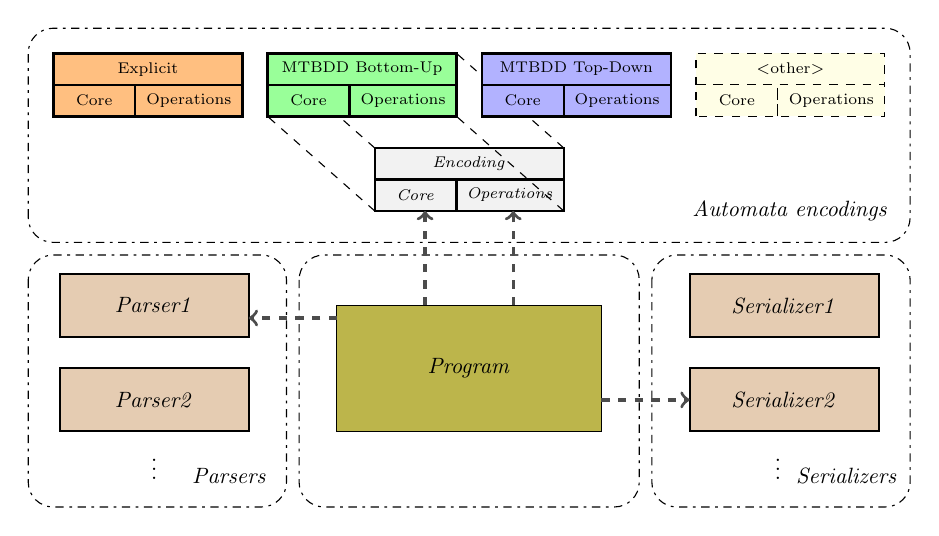
\begin{tikzpicture}
[
  scale=1,
  transform shape,
	gen/.style={thick,fill=gray!10},
	expl/.style={thick,fill=orange!50},
	bu/.style={thick,fill=green!40},
	td/.style={thick,fill=blue!30},
	other/.style={fill=yellow!10,dashed}
]

% encodings
\draw[dashed] (0,1) -- (-1.7,2.5);
\draw[dashed] (0,0) -- (-1.7,1.5);
\draw[dashed] (3,1) -- (1.3,2.5);

\draw (0,0.5) rectangle +(3, 0.5) [gen] node[midway] {\textit{\scriptsize{Encoding}}};
\draw (0,0) rectangle +(1.3, 0.5) [gen] node[midway] {\textit{\scriptsize{Core}}};
\draw (1.3,0) rectangle +(1.7, 0.5) [gen] node[midway] {\textit{\scriptsize{Operations}}};

\draw (-5.1,2) rectangle +(3, 0.5) [expl] node[midway] {\scriptsize{Explicit}};
\draw (-5.1,1.5) rectangle +(1.3, 0.5) [expl] node[midway] {\scriptsize{Core}};
\draw (-3.8,1.5) rectangle +(1.7, 0.5) [expl] node[midway] {\scriptsize{Operations}};

\draw (-1.7,2) rectangle +(3, 0.5) [bu] node[midway] {\scriptsize{MTBDD Bottom-Up}};
\draw (-1.7,1.5) rectangle +(1.3, 0.5) [bu] node[midway] {\scriptsize{Core}};
\draw (-0.4,1.5) rectangle +(1.7, 0.5) [bu] node[midway] {\scriptsize{Operations}};

\draw (1.7,2) rectangle +(3, 0.5) [td] node[midway] {\scriptsize{MTBDD Top-Down}};
\draw (1.7,1.5) rectangle +(1.3, 0.5) [td] node[midway] {\scriptsize{Core}};
\draw (3.0,1.5) rectangle +(1.7, 0.5) [td] node[midway] {\scriptsize{Operations}};

\draw (5.1,2) rectangle +(3, 0.5) [other] node[midway] {\scriptsize{$<$other$>$}};
\draw (5.1,1.5) rectangle +(1.3, 0.5) [other] node[midway] {\scriptsize{Core}};
\draw (6.4,1.5) rectangle +(1.7, 0.5) [other] node[midway] {\scriptsize{Operations}};

\draw[dashed] (3,0) -- (1.3,1.5);

\draw[rounded corners=9,dash pattern=on 3pt off 2pt on 1pt off 2pt] (-5.5,-0.5) rectangle +(14,3.4);

\draw (6.6,0) node {\textit{Automata encodings}};


% parsers
\draw (-5,-2) rectangle +(3, 1) [gen,fill=brown!40] node[midway] (parser1) {\textit{Parser1}};
\draw (-5,-3.5) rectangle +(3, 1) [gen,fill=brown!40] node[midway] {\textit{Parser2}};
\draw (-3.5,-4) node {$\vdots$};

\draw[rounded corners=9,dash pattern=on 3pt off 2pt on 1pt off 2pt] (-5.5,-0.7) rectangle +(4.1,-4);
\draw (-2.3,-4.2) node {\textit{Parsers}};

% serializers
\draw (5,-2) rectangle +(3, 1) [gen,fill=brown!40] node[midway] {\textit{Serializer1}};
\draw (5,-3.5) rectangle +(3, 1) [gen,fill=brown!40] node[midway] {\textit{Serializer2}};
\draw (6.4,-4) node {$\vdots$};

\draw[rounded corners=9,dash pattern=on 3pt off 2pt on 1pt off 2pt] (4.4,-0.7) rectangle +(4.1,-4);
\draw (7.5,-4.2) node {\textit{Serializers}};

% program
\draw[rounded corners=9,dash pattern=on 3pt off 2pt on 1pt off 2pt] (-1.2,-0.7) rectangle +(5.4,-4);

\draw[fill=olive!60] (-0.6,-1.5) rectangle (3.6,-3.5) node[midway] {\textit{Program}};

\draw[very thick,dashed,->,black!70] (-0.6,-1.7) -- (-2,-1.7);
\draw[very thick,dashed,->,black!70] (3.6,-3) -- (5,-3);
\draw[very thick,dashed,->,black!70] (0.8,-1.5) -- (0.8,0);
\draw[very thick,dashed,->,black!70] (2.2,-1.5) -- (2.2,0);

\end{tikzpicture}

		\caption{The main concept of \vata. Figure is taken from \cite{libvata}.}
		\label{fig:vata}
\end{center}
\end{figure}

A \emph{program} (e.g. cli of VATA) employing the three parts of \vata\ works as follows.
An input automaton is loaded by one of the parsers to an intermediate representation.
The wrapping program chooses an internal encoding of NTA to which is automaton stored
from intermediate encoding (note that it is also
possible to create automaton in the chosen encoding directly using API provided by VATA).
Then the automaton is processed by applying the operations implemented by a module of the chosen encoding.
Finally, the automaton can be serialized to an output format.
When one wants to add her own the encoding
then she needs to implement only a core of encoding (with API for creating automaton itself)
and needed operations over TA and can employ already implemented parses and serializers in \vata.

\subsection{Implemented NTA Encodings}

It was mentioned that there are currently implemented two representation of TA and we will are describe both
of them in the following subsection.

Using the \emph{explicit encoding} of NTA transition relation is represented by a hierarchy
of the hash tables as it is shown in Figure \ref{fig:explnta}.
The first level of the hash tables hierarchy (\emph{top-level look-up tables}) maps each state $q$ to 
the second level of the hash tables hierarchy (\emph{transition cluster}).
There are stored all symbols presented in the transition with state $q$ at the left-handed side.
Each symbol $a$ in a transition cluster is mapped to a pointer to a set in the third level of hierarchy (\emph{sets of pointers to tuple}).
The set contains pointers to the tuples which are at the right-handed side in
a transition with $q$ at the left-handed side and with $a$ as symbol.
The tuples are stored at a special set where every tuples is stored only once.
Note that it is also possible to share the part of the transition relation between different automata.
This brings the higher efficiency in space complexity of implementation.
Module for explicit encoding also stores explicitly a set of the final states of a NFA.
On the other side, it does not explicitly store a set of all states because it can be obtained from the transition relation.

\begin{figure}[bt]
\begin{center}
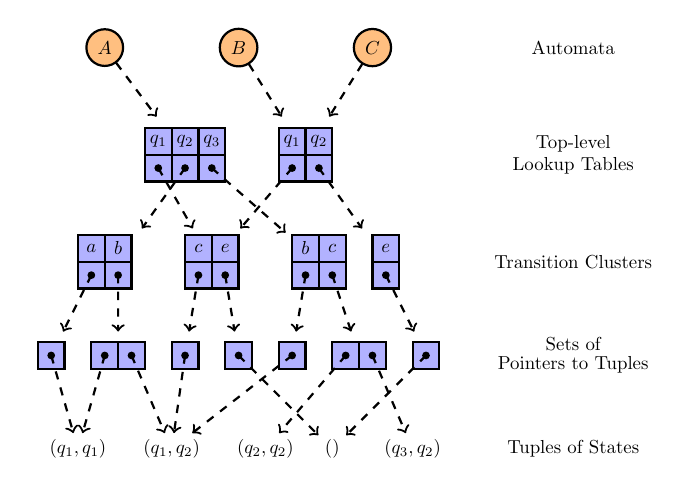
\begin{tikzpicture}
[
  scale=0.85,
  transform shape,
	gen/.style={thick,fill=gray!10},
	expl/.style={thick,fill=orange!50},
	bu/.style={thick,fill=green!40},
	td/.style={thick,fill=blue!30},
	other/.style={fill=yellow!10,dashed}
]

\node at(10,2) {Automata};

\node[expl,circle,draw] (aA) at(1.25,2) {\textit{$A$}};
\node[expl,circle,draw] (aB) at(3.75,2) {\textit{$B$}};
\node[expl,circle,draw] (aC) at(6.25,2) {\textit{$C$}};


\node at(10,0) {\shortstack{Top-level\\ Lookup Tables}};

\node[minimum size=40pt](table1) at (2.75,0) {};
\draw (2,0) rectangle +(0.5, .5) [td] node[midway] {\textit{$q_1$}};
\draw (2,-.5) rectangle +(0.5, .5) [td] node[midway] {};
\draw (2.5,0) rectangle +(0.5, .5) [td] node[midway] {\textit{$q_2$}};
\draw (2.5,-.5) rectangle +(0.5, .5) [td] node[midway] {};
\draw (3,0) rectangle +(0.5, .5) [td] node[midway] {\textit{$q_3$}};
\draw (3,-.5) rectangle +(0.5, .5) [td] node[midway] {};

\node[minimum size=40pt](table2) at (5,0) {};
\draw (4.5,0) rectangle +(0.5, .5) [td] node[midway] {\textit{$q_1$}};
\draw (4.5,-.5) rectangle +(0.5, .5) [td] node[midway] {};
\draw (5,0) rectangle +(0.5, .5) [td] node[midway] {\textit{$q_2$}};
\draw (5,-.5) rectangle +(0.5, .5) [td] node[midway] {};


\draw[->,thick,dashed] (aA) -- (table1);
\draw[->,thick,dashed] (aB) -- (table2);
\draw[->,thick,dashed] (aC) -- (table2);


\node at(10,-2) {Transition Clusters};

\node[minimum size=35](cluster1) at (1.5,-2) {};
\draw (0.75,-2) rectangle +(0.5, .5) [td] node[midway] {\textit{$a$}};
\draw (0.75,-2.5) rectangle +(0.5, .5) [td] node[midway] {};
\draw (1.25,-2) rectangle +(0.5, .5) [td] node[midway] {\textit{$b$}};
\draw (1.25,-2.5) rectangle +(0.5, .5) [td] node[midway] {};

\node[minimum size=35pt](cluster2) at (3.25,-2) {};
\draw (2.75,-2) rectangle +(0.5, .5) [td] node[midway] {\textit{$c$}};
\draw (2.75,-2.5) rectangle +(0.5, .5) [td] node[midway] {};
\draw (3.25,-2) rectangle +(0.5, .5) [td] node[midway] {\textit{$e$}};
\draw (3.25,-2.5) rectangle +(0.5, .5) [td] node[midway] {};

\node[minimum size=35pt](cluster3) at (5.25,-2) {};
\draw (4.75,-2) rectangle +(0.5, .5) [td] node[midway] {\textit{$b$}};
\draw (4.75,-2.5) rectangle +(0.5, .5) [td] node[midway] {};
\draw (5.25,-2) rectangle +(0.5, .5) [td] node[midway] {\textit{$c$}};
\draw (5.25,-2.5) rectangle +(0.5, .5) [td] node[midway] {};

\node[minimum size=35pt](cluster4) at (6.5,-2) {};
\draw (6.25,-2) rectangle +(0.5, .5) [td] node[midway] {\textit{$e$}};
\draw (6.25,-2.5) rectangle +(0.5, .5) [td] node[midway] {};


\draw[thick,fill=black] (2.25,-0.25) circle (0.5mm);
\draw[->,thick,dashed] (2.25,-.25) -- (cluster2);

\draw[thick,fill=black] (2.75,-0.25) circle (0.5mm);
\draw[->,thick,dashed] (2.75,-.25) -- (cluster1);

\draw[thick,fill=black] (3.25,-0.25) circle (0.5mm);
\draw[->,thick,dashed] (3.25,-.25) -- (cluster3);

\draw[thick,fill=black] (4.75,-0.25) circle (0.5mm);
\draw[->,thick,dashed] (4.75,-.25) -- (cluster2);

\draw[thick,fill=black] (5.25,-0.25) circle (0.5mm);
\draw[->,thick,dashed] (5.25,-.25) -- (cluster4);


\node at(10,-3.75) {\shortstack{Sets of\\ Pointers to Tuples}};

\node[minimum size=25pt](set1) at (0.25,-3.75) {};
\draw (0,-4) rectangle +(0.5, .5) [td] node[midway] {};

\node[minimum size=25pt](set2) at (1.5,-3.75) {};
\draw (1,-4) rectangle +(0.5, .5) [td] node[midway] {};
\draw (1.5,-4) rectangle +(0.5, .5) [td] node[midway] {};

\node[minimum size=25pt](set3) at (2.75,-3.75) {};
\draw (2.5,-4) rectangle +(0.5, .5) [td] node[midway] {};

\node[minimum size=25pt](set4) at (3.75,-3.75) {};
\draw (3.5,-4) rectangle +(0.5, .5) [td] node[midway] {};

\node[minimum size=25pt](set5) at (4.75,-3.75) {};
\draw (4.5,-4) rectangle +(0.5, .5) [td] node[midway] {};

\node[minimum size=25pt](set6) at (6,-3.75) {};
\draw (5.5,-4) rectangle +(0.5, .5) [td] node[midway] {};
\draw (6,-4) rectangle +(0.5, .5) [td] node[midway] {};

\node[minimum size=25pt](set7) at (7.25,-3.75) {};
\draw (7,-4) rectangle +(0.5, .5) [td] node[midway] {};


\draw[thick,fill=black] (1,-2.25) circle (0.5mm);
\draw[->,thick,dashed] (1,-2.25) -- (set1);

\draw[thick,fill=black] (1.5,-2.25) circle (0.5mm);
\draw[->,thick,dashed] (1.5,-2.25) -- (set2);

\draw[thick,fill=black] (3,-2.25) circle (0.5mm);
\draw[->,thick,dashed] (3,-2.25) -- (set3);

\draw[thick,fill=black] (3.5,-2.25) circle (0.5mm);
\draw[->,thick,dashed] (3.5,-2.25) -- (set4);

\draw[thick,fill=black] (5,-2.25) circle (0.5mm);
\draw[->,thick,dashed] (5,-2.25) -- (set5);

\draw[thick,fill=black] (5.5,-2.25) circle (0.5mm);
\draw[->,thick,dashed] (5.5,-2.25) -- (set6);

\draw[thick,fill=black] (6.5,-2.25) circle (0.5mm);
\draw[->,thick,dashed] (6.5,-2.25) -- (set7);


\node at(10,-5.5) {Tuples of States};

\node(tup1) at (0.75,-5.5) {$(q_1, q_1)$};
\node(tup2) at (2.5,-5.5) {$(q_1, q_2)$};
\node(tup3) at (4.25,-5.5) {$(q_2, q_2)$};
\node(tup4) at (7,-5.5) {$(q_3, q_2)$};
\node(tup5) at (5.5,-5.5) {$()$};

\draw[thick,fill=black] (0.25,-3.75) circle (0.5mm);
\draw[->,thick,dashed] (0.25,-3.75) -- (tup1);

\draw[thick,fill=black] (1.25,-3.75) circle (0.5mm);
\draw[->,thick,dashed] (1.25,-3.75) -- (tup1);

\draw[thick,fill=black] (1.75,-3.75) circle (0.5mm);
\draw[->,thick,dashed] (1.75,-3.75) -- (tup2);

\draw[thick,fill=black] (2.75,-3.75) circle (0.5mm);
\draw[->,thick,dashed] (2.75,-3.75) -- (tup2);

\draw[thick,fill=black] (3.75,-3.75) circle (0.5mm);
\draw[->,thick,dashed] (3.75,-3.75) -- (tup5);

\draw[thick,fill=black] (4.75,-3.75) circle (0.5mm);
\draw[->,thick,dashed] (4.75,-3.75) -- (tup2);

\draw[thick,fill=black] (5.75,-3.75) circle (0.5mm);
\draw[->,thick,dashed] (5.75,-3.75) -- (tup3);

\draw[thick,fill=black] (6.25,-3.75) circle (0.5mm);
\draw[->,thick,dashed] (6.25,-3.75) -- (tup4);

\draw[thick,fill=black] (7.25,-3.75) circle (0.5mm);
\draw[->,thick,dashed] (7.25,-3.75) -- (tup5);


\end{tikzpicture}

	\caption{Explicit representation of NTA in \vata. Figure is taken from \cite{libvata}}.
	\label{fig:explnta}
\end{center}
\end{figure}

\begingroup
\tikzset{every picture/.style={scale=0.8}}%
\begin{figure}[bt]
	\centering
	\begin{subfigure}{.5\textwidth}
		\centering
		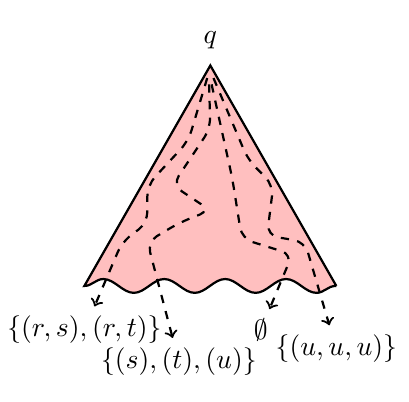
\begin{tikzpicture}
[]
\useasboundingbox (-2.9,-4.9) rectangle (2.7,0.6);

<<<<<<< HEAD
=======

>>>>>>> fcad047018e021c44f6be41eab656d5ec3da0ca5
%\draw[thick,fill=blue!40] (3,-5) -- (0,0) -- (-3,-5) .. controls (-1,-3.5) and (1,-6.5) .. (3,-5);
\draw[thick,fill=pink] (2,-3.5) -- (0,0) -- (-2,-3.5) decorate[decoration=snake,segment length=22] { -- cycle};

\node at (0,0.4){$q$};

\node(set1) at (-2,-4.2) {$\{(r,s),(r, t)\}$};
\node(set2) at (-0.5,-4.7) {$\{(s), (t), (u)\}$};
\node(set3) at (0.8,-4.2) {$\emptyset$};
\node(set4) at (2,-4.5) {$\{(u, u, u)\}$};

\draw[->,thick,dashed,rounded corners] (-0.05,-0.2) -- (-0.35,-1.2) -- (-1,-1.9) -- (-1,-2.5) -- (-1.4,-2.8) -- (set1);
\draw[->,thick,dashed,rounded corners] (-0.02,-0.3) -- (0,-1) -- (-0.6,-1.9) -- (0,-2.3) -- (-0.5,-2.5) -- (-1,-2.8) -- (set2);
\draw[->,thick,dashed,rounded corners] (0.02,-0.3) -- (0.35,-1.8) -- (0.5,-2.75) -- (1.3,-3) -- (set3);
\draw[->,thick,dashed,rounded corners] (0.05,-0.2) -- (0.6,-1.5) -- (1,-1.9) -- (0.9,-2.7) -- (1.5,-2.8) -- (set4);



\end{tikzpicture}
		\caption{MTBDD Top-down representation of a NTA. Image is taken from \cite{libvata}.}
		\label{fig:mtbdd_td}
	\end{subfigure}%
	~
	\begin{subfigure}{.5\textwidth}
	\centering
	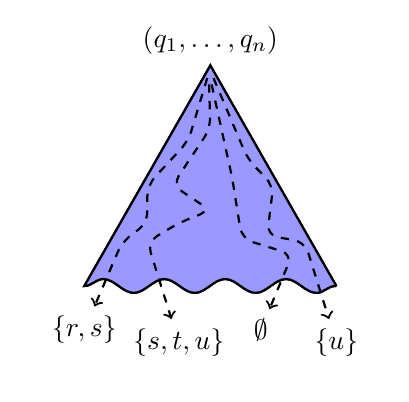
\begin{tikzpicture}
[]
\useasboundingbox (-2.9,-4.9) rectangle (2.7,0.6);
<<<<<<< HEAD
%\draw[thick,fill=blue!40] (3,-5) -- (0,0) -- (-3,-5) .. controls (-1,-3.5) and (1,-6.5) .. (3,-5);
\draw[thick,fill=blue!40] (2,-3.5) -- (0,0) -- (-2,-3.5) decorate[decoration=snake,segment length=22] { -- cycle};

=======

%\draw[thick,fill=blue!40] (3,-5) -- (0,0) -- (-3,-5) .. controls (-1,-3.5) and (1,-6.5) .. (3,-5);
\draw[thick,fill=blue!40] (2,-3.5) -- (0,0) -- (-2,-3.5) decorate[decoration=snake,segment length=22] { -- cycle};


>>>>>>> fcad047018e021c44f6be41eab656d5ec3da0ca5
\node at (0,0.4){$(q_1,\dots, q_n)$};

\node(set1) at (-2,-4.2) {$\{r,s\}$};
\node(set2) at (-0.5,-4.4) {$\{s, t, u\}$};
\node(set3) at (0.8,-4.2) {$\emptyset$};
\node(set4) at (2,-4.4) {$\{u\}$};

\draw[->,thick,dashed,rounded corners] (-0.05,-0.2) -- (-0.35,-1.2) -- (-1,-1.9) -- (-1,-2.5) -- (-1.4,-2.8) -- (set1);
\draw[->,thick,dashed,rounded corners] (-0.02,-0.3) -- (0,-1) -- (-0.6,-1.9) -- (0,-2.3) -- (-0.5,-2.5) -- (-1,-2.8) -- (set2);
\draw[->,thick,dashed,rounded corners] (0.02,-0.3) -- (0.35,-1.8) -- (0.5,-2.75) -- (1.3,-3) -- (set3);
\draw[->,thick,dashed,rounded corners] (0.05,-0.2) -- (0.6,-1.5) -- (1,-1.9) -- (0.9,-2.7) -- (1.5,-2.8) -- (set4);



\end{tikzpicture}
	\caption{MTBDD Bottom-up representation of a NTA. Image is taken from \cite{libvata}.}
	\label{fig:mtbdd_bu}
	\end{subfigure}%
\caption{Semi-symbolic encoding of tree automata.}
\label{fig:symnta}
\end{figure}
\endgroup

The other already implemented encoding is a \emph{semi-symbolic} one
based on VATA own implementation of the MTBDD package.
This encoding is efficient mainly for TA with the large alphabets.
Since semi-symbolic encoding and MTBDD are not in the aim of this thesis
they are not going to be described in detail
and we refer rather to \cite{mt:lengal}.
The main principle of the semi-symbolic encoding is shown in Figure \ref{fig:symnta}.
First of all it is necessary to distinguish between (a) top-down and (b) bottom-up variants of this encoding.
The first one maps each state $q$ of a NTA using MTBDD to the sets of the tuples of states such that that it is possible
to make transition from $q$ under a symbol $a$ to a tuple in appropriate set (each set of tuples is dedicated
to one symbol under which it is possible to make transition from $q$).
The former one symmetrically maps each n-tuple $(q_1 \cdots q_n)$ of a NTA using MTBDD to the sets of states.
Each such a set $S$ is dedicated to a symbol $a$ of the NTA and
it contains states such that there exists a transition
with $(q_1 \cdots q_n)$ at the right-handed side and symbol $a$ and state from the set $S$ at the left-handed side.
The final state set of a NTA is again represented by explicit set in the both variants.
A state set is not stored explicitly because one can obtain it from the transition relation.
The symbols are encoded (as binary strings) in MTBDD.

All of the mentioned encodings currently support efficient language inclusion checking using algorithm
from \cite{tacas10}.
On the other side, the other operations are not currently implemented by all encodings.
The full enumeration of the supported operations for the particular encodings is given in Table \ref{tab:vataop}.

\begin{table}[bt]
	\begin{center}
		\catcode`\-=12
		\begin{tabular}{| l | c | c | c |} \hline
		& {\textbf{Explicit}} & \multicolumn{2}{|c|}{\textbf{Semi-symbolic}} \\ \cline{2-4}
		\textbf{Operation} & \textbf{top-down} & \textbf{bottom-up} & \textbf{top-down} \\ \hline
		Union & $+$ & $+$ & $+$ \\
		Intersection & $+$ & $+$ & $+$ \\
		Complement (experimental) & $+$ & $+$ & $+$ \\
		Removing useless states & $+$ & $+$ & $+$ \\
		Removing unreachable states & $+$ & $+$ & $+$ \\
		Simulation & $+$ & $-$ & $-$ \\
		Downward Inclusion  & $+$ & $+$ & $-$ \\ 
		Upward Inclusion  & $+$ & $-$ & $-$ \\ 
		Simulation over LTS (Labeled Transitions System) & $+$ & $-$ & $-$ \\ \hline
		\end{tabular}
	\caption{Table of supported operations over NTA by particular encodings implemented in \vata.
	Table is taken from \cite{bt:hruska}.}
	\label{tab:vataop}
	\end{center}
\end{table}


\section{Forester}
\label{sec:FA}

Forester is an open source tool written in C++ for verification of programs manipulating
complex dynamic data structures.
It currently supports the programs in the C language.
Forester is distributed as a \emph{GCC} plugin under GPL license, version 3,
and it can be obtained from its official website \cite{www:forester}.

\subsection{Design}

Forester is implemented as a GCC plugin however it does not analyze directly intermediate code of GCC called GIMPLE.
It uses the Code Listener infrastructure \cite{cl11}
that provides fronted over the GIMPLE format.

The high level overview of the process performed by
Forester is shown in Figure \ref{fig:fa_exec}. 
Forester starts the analysis of a program by translation of the intermediate
code representation provided by Code Listener to its own microcode.
The microcode represents each program statement by one
or a few instructions associated with the abstract transformers.
Symbolic execution is then executed over this microcode.
Abstract domain represented by FA (which are also the core part of a symbolic state) is gradually transformed by the abstract transformers
represented by the microcode instructions during the symbolic execution.
When Forester detects an error the symbolic execution is aborted and
the analyzed program is claimed as incorrect one.
During the symbolic execution Forester gradually checks whether there is no left garbage.
The presence of garbage is also checked at the end of symbolic execution.
If the program is garbage free and free then a shape invariant has been found
and the analyzed program is determined as correct.

\begin{figure}[bt]
	\begin{center}
		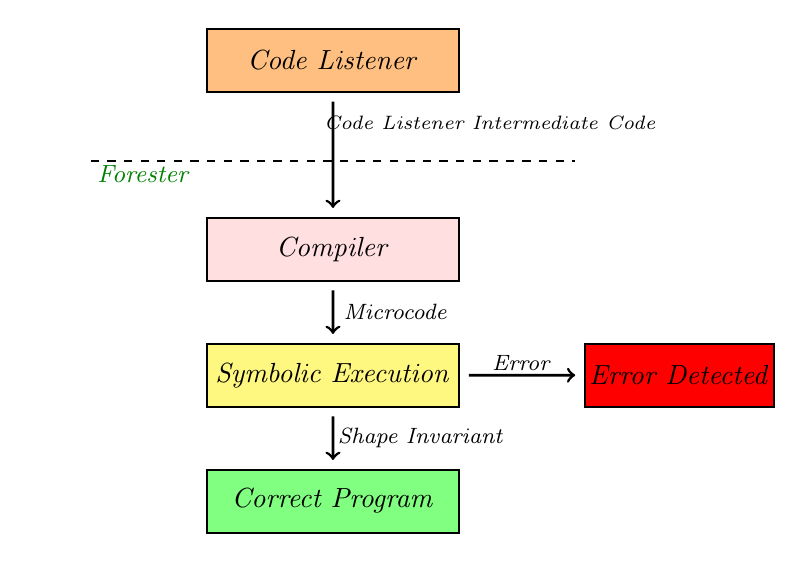
\begin{tikzpicture}[
  cl/.style={thick,fill=orange!50},
  red/.style={thick,fill=Red},
  detection/.style={thick,fill=blue!50},
  compiler/.style={thick,fill=pink!50},
  symexec/.style={thick,fill=yellow!50},
  success/.style={thick,fill=green!50},
  arrow/.style={->,line width=1pt}
  ]

\node (InputNode) at(1.3,10.9) {};
\node (InputDown) at(1.3,10.8) {};

\draw (4,11) rectangle +(4, 1) [cl] node[midway] {\textit{Code Listener}};
\node (CLDown) at(6,11) {};

\draw (4,8) rectangle +(4, 1) [compiler] node[midway] {\textit{Compiler}};
\node (CompUp) at(6,9) {};
\node (CompDown) at(6,8) {};

\draw (4,6) rectangle +(4, 1) [symexec] node[midway] {\textit{Symbolic Execution}};
\node (SymexUp) at(6,7) {};
\node (SymexDown) at(6,6) {};
\node (SymexRight) at(8,6.5) {};

\draw (10,6) rectangle +(3, 1) [red] node[midway] {\textit{Error Detected}};
\node (ErrLeft) at(10,6.5) {};

\draw (4,4) rectangle +(4, 1) [success] node[midway] {\textit{Correct Program}};
\node (CPUp) at(6,5) {};

\draw [arrow] (CLDown) -- (CompUp);
\draw [arrow] (CompDown) -- (SymexUp);
\draw [arrow] (SymexRight) -- (ErrLeft);
\draw [arrow] (SymexDown) -- (CPUp);

\node (LeftFAStart) at(2,9.9) {};
\node (RightFAStart) at(10,9.9) {};
\draw [dashed, line width = 1pt] (LeftFAStart) -- (RightFAStart);

\node (Input) at(8.5,10.5) {\textcolor{Black}{\scriptsize{\textit{Code Listener Intermediate Code}}}};
\node (Input) at(7,7.5) {\textcolor{Black}{\footnotesize{\textit{Microcode}}}};
\node (Input) at(9,6.7) {\textcolor{Black}{\footnotesize{\textit{Error}}}};
\node (Input) at(7.4,5.5) {\textcolor{Black}{\footnotesize{\textit{Shape Invariant}}}};

\node (Input) at(3,9.7) {\textcolor{Green}{\small{\textit{Forester}}}};

\end{tikzpicture}

	\end{center}
	\caption{High level overview of Forester program analysis.}
	\label{fig:fa_exec}
\end{figure}

We further deeper describe the conceptual design of Forester (which is shown in Figure~\ref{fig:fa_design})
and the relations between its modules.
Note that implementation of Forester is not explicitly separated to the stand-alone compilation modules so the notion of the modules
used in following text is more abstract to provide reader basic summary of the Forester design.
One module could be e.g. a set of closely related classes with a similar purpose.
As it was mentioned above, the Code Listener representation of GCC intermediate code is mainly used by Forester \emph{Compiler} module.
Compiler then converts Code Listener instructions to Forester own \emph{Microcode Instructions}
and creates their list over which the \emph{Symbolic Execution} is performed.
Symbolic execution then executes the microcode instructions (abstract transformers)
which manipulates \emph{Symbolic State} and
\emph{Forest Automata} included in the symbolic states.
Symbolic execution requires \emph{Symbol Context} which is created for each function and also for global space.
It keeps information about the variables used in the current scope,
the function arguments and the stack frame layout.
A symbolic state provides information about the state of the heap represented
by the FA and it also keeps the information about
the corresponding microcode instructions.
\emph{Forest Automata} module provides the methods
for manipulation with FA during the verification procedure.
The operations such as normalization or abstraction over FA are not the part of the module
containing FA implementation but are provided as the classes taking FA as parameters.
So these operations can be understood as another module \emph{Operations over Forest Automata}.
Forester currently has its own implementation of \emph{Tree Automata}.
It is very lightweighted and containing the optimized
operations directly for the Forester purposes.
One of them is operation for the language inclusion checking using the simulation relation
and the efficiency is also crucial for the performance.
The advantage of this implementation is its simplicity and the efficiency raising
from the optimization the implementation to suit the Forester needs.
On the other side, it is not easy to maintain such a optimized implementation.
Especially, when one considers that there is still progress
in the field of design of the efficient algorithms and any improvement of
an algorithm brings often much higher efficiency
then smaller implementation optimization.

\begin{figure}[bt]
	\begin{center}
		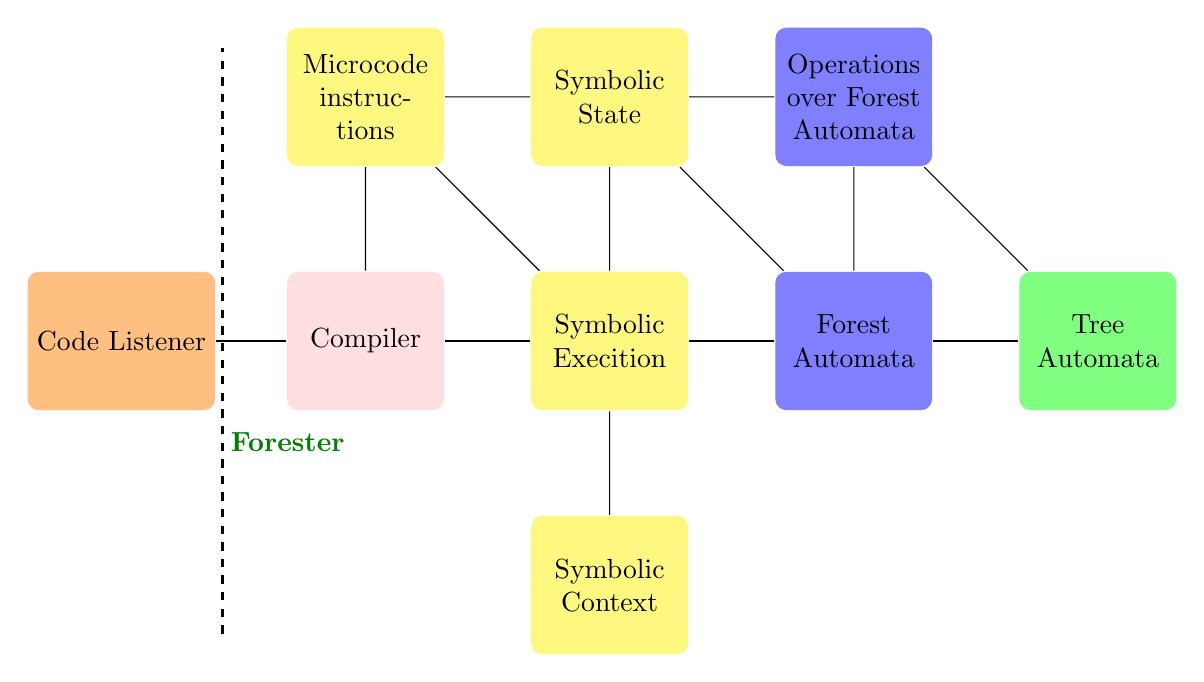
\begin{tikzpicture}[
  scale=0.8,
  node distance = 3.1cm,
  block_cl/.style={rectangle, text centered, rounded corners, thick, fill=orange!50,
    minimum height = 5em, minimum width = 3em},
  block_compiler/.style={rectangle, text centered, rounded corners, thick, fill=pink!50,
    minimum height = 5em, minimum width = 3em, text width = 5em},
  block_symex/.style={rectangle, text centered, rounded corners, thick, fill=yellow!50,
    minimum height = 5em, minimum width = 3em, text width = 5em},
  block_fa/.style={rectangle, text centered, rounded corners, thick, fill=blue!50,
    minimum height = 5em, minimum width = 3em, text width = 5em},
  block_ta/.style={rectangle, text centered, rounded corners, thick, fill=green!50,
    minimum height = 5em, minimum width = 3em, text width = 5em},
  line/.style={draw, -}
  ]

\node [block_cl] (cl) {Code Listener};
\node [block_compiler, right of=cl] (compiler) {Compiler};
\node [block_symex, above of=compiler] (microcode) {Microcode instructions};
\node [block_symex, right of=compiler] (symex) {Symbolic Execition};
\node [block_symex, above of=symex] (symstate) {Symbolic State};
\node [block_symex, below of=symex] (symcnt) {Symbolic Context};

\node [block_fa, right of=symex] (fa) {Forest Automata};
\node [block_fa, above of=fa] (faop) {Operations over Forest Automata};

\node [block_ta, right of=fa] (ta) {Tree Automata};

\path [line] (cl) -- (compiler);
\path [line] (microcode) -- (compiler);
\path [line] (symex) -- (compiler);
\path [line] (symex) -- (symstate);
\path [line] (symex) -- (symcnt);
\path [line] (symex) -- (fa);
\path [line] (symstate) -- (fa);
\path [line] (microcode) -- (symex);
\path [line] (fa) -- (faop);
\path [line] (fa) -- (ta);
\path [line] (symstate) -- (faop);
\path [line] (faop) -- (ta);
\path [line] (microcode) -- (symstate);

\node (LeftFAStart) at(2,-6) {};
\node (RightFAStart) at(2,6) {};
\draw [dashed, line width = 1pt] (LeftFAStart) -- (RightFAStart);
\node (Input) at(3.3,-2) {\textcolor{Green}{\textbf{Forester}}};

\end{tikzpicture}

	\end{center}
	\caption{Conceptual design of Forester.}
	\label{fig:fa_design}
\end{figure}

Note, this is just the conceptual high level view of the Forester design.
A real implementation is much more complicated (e.g. Forest automata are implemented by two classes: \emph{FA} and \emph{FAE})
and full of the technical details.
A full description of the implementation is also not the aim of this text.

It was already mentioned that the substitution of the underlying TA implementation with the
VATA library could bring some improvements.
The first one is the easier maintenance of the library where
the state-of-the-art algorithms are implemented and optimized
in comparison with the hardwired implementation.
Since VATA and Forester are developed by the same developers it also easy to add
to VATA the operations needed by Forester.
The narrow interface between TA library and the rest of Forester
also improves code quality of Forester in the sense of modularity, maintainability and code organization.
These benefits led us to implement the version of Forester using VATA
further described in Section \ref{ch:fova}.


\subsection{Implementation of Forest Automata Concepts}
\label{subsec:faimpl}

This subsection describes an implementation of the forest automata 
based verification procedure in Forester.
The core of the forest automata module is class {\tt FA}.
The implementation corresponds with the definitions given in Chapter \ref{ch:prel}.
Class FA has a data member representing a vector of tree automata $(t_1 \cdots t_n)$.
It also has a data member keeping a reference to an automaton representing the global variables
and a reference to the automata representing the local variables of the actually executed function. %TODO define ABP
The basic operations over an FA (like adding or removing a TA from an FA) are encapsulated in class FA.
The another class providing operations over FA is class {\tt FAE}. 

The labels of the TA transitions are represented by the structure {\tt NodeLabel}.
It can be defined as a tuple $NL=(T,V)$.
This structure contains a data member $T$ determining the type of the root node of a transition
(whether it is a general node, a data node or~a node containing a vector of data).
A value $V$ related to the type of the node is also stored as a data member of the structure.

As it was already mentioned, the forest automata are further used in the representation of a symbolic state.
An implementation of the representation of a symbolic state is in class {\tt SymState}.
This class keeps a reference to a Forester microcode instruction $I$ to which the~symbolic state corresponds.
It has a data member that is a pointer to a forest automaton~$F$ (an instance of class {\tt FAE})
representing the actual memory shape in the symbolic state.
Another data member of class SymState is a set of registers $\regsset$.
We denote set $\regsset$ by $\regs$. 
The register can be local or global.
There are two global registers.
The first one contains a reference to the forest automata modelling
the global state, e.g., the block of global variables in the symbolic state.
The other then represents the allocated memory of the actually executed function.
The local registers serve as temporary memory used in
the microcode instructions for the data manipulation.
Putting together the data members of class {\tt SymState},
we can define symbolic state formally as a triple $S=\symstate{F}{\regs}{I}$.

The values of the registers are instances of a structure {\tt Data}.
We can formally define structure Data as $\ddata$ where
$T$ is a data type,
$S \in \natnum$ is a size of data,
$V$ is a value of type $T$,
$MB=(D_1 \cdots D_n)$ represents nested data if they are present (this is the case when $D$ represents a data structure)
and $D_i$ is another instance of data.
$T$ can be one of the following data types: pointer, reference to a TA, integer, boolean,
structure or generally some other data type.
$T$ can be also undefined or a state with the type that is unknown.
We describe in detail one of the types\,---\,the root reference.
Its values are defined as $RR=({\tt Root},{\tt Displ})$
where ${\tt Root} \in \natnum$ is an index of a tree automaton in $F$
and ${\tt Displ} \in \natnum$ is an index of a selector in a structured label of
the transition with ${\tt Root}$ at the left-handed side.
The~operations for manipulation with a symbolic state are partially provided by class {\tt SymState}
and some additional operations are provided by class {\tt VirtualMachine}.

We already described the data structures used for the implementation of the forest automata concepts
and the related symbolic execution.
The symbolic execution using this data structures is realized by gradually appending
and removing the symbolic states from a queue.
It implementation is in class \emph{SymExec}.
When a symbolic state is taken from the queue a microcode instruction contained in
the symbolic state is executed.
Some of the instructions during its execution appends a new symbolic state to the queue.
Symbolic execution finishes when the queue is empty.
The microcode instructions executed during the symbolic execution are described in the following section.

\subsection{The Microcode Instructions}
\label{subsec:microinstr}

This sections provides a description of the Forester microcode instructions
which correspond to the abstract transformers in abstraction interpretation.
First, we introduce some examples how the C statements are translated
to the corresponding Forester microcode instructions, then we define the instructions
more formally and we give a complete list of them.

Consider the following data structure that is an implementation of singly-linked list.
	\begin{quote}
	\begin{verbatim}
	struct T {
      struct T* next;
      int data;
	};

	\end{verbatim}
	\end{quote}
	
	Consider also two variables \code{struct T *x, *y} used in the next examples.
	Note that all constants used in the examples are dependent on a concrete Forester
	run and they are chosen randomly in this text.
	The syntax of the instructions in the examples is following:
	$$ op\ r_0,\ r_1,\ r_2$$
	where $op$ is a name of a instruction,
	$r_0, r_1, r_2$ are operands such that $r_0$ is a destination register,
	$r_1$ and $r_2$ are the source registers.
	The instructions do not require all three registers as the parameters.
	%Indeed, the most of them have just two.
	A constant may be also used as an operand instead of the registers as a parameter.
	When $[r+c]$ is used as an operand then the instruction dereferences a root reference in register $r$.
	In this case, the instruction accesses directly a selector with the displacement $c$ in a label of the transition with
	root at the left-handed side.
	We will further consider the selector in a label of transition with
	the referenced root at left-handed side if it is not stated otherwise.
	In the following text the registers $r_1,\ldots,r_n$ are local ones.
	$GLOB$ and $ABP$ are global registers such that $GLOB$ register contains reference to a FA representing
	global variables and $ABP$ register contains reference to a FA representing local memory.

\bexmp
	The statement \codix{x = (struct T*) malloc(sizeof(struct T));} is translated
	to these microcode instructions:
	\begin{quote}
	\begin{verbatim}
	1: mov_reg r0, (int)4
	2: alloc r0, r0
	3: node_create r0, r0, next[0:4:+0]
	4: mov_reg r1, ABP + 0
	5: mov_reg [r1 + 12], r0    
	6: check
	\end{verbatim}
	\end{quote}

	Firstly the size of the new allocated data (in this case the size is $4$)
	is stored in the register $0$ at line~$1$.
	Then the new instance of structure {\tt Data} is created and stored to register $0$ at line $2$.
	A~new TA $t$ is created at line $3$.
	The TA $t$ has one transition from the root with a label that consists one pointer selector {\tt next} whose
	displacement in the label is $0$ and the size is $4$.
	The displacement defines the order of the selector in the label.
	The instruction \codix{node} stores a root reference to $t$ to register $0$.
	Finally lines $4$ a $5$ add a root reference pointing to $t$ to a FA representing
	a memory state of the actually executed function (which is in this case the function {\tt main}).
	In this case a selector related to the pointer x has displacement $12$ in the label of TA
	representing the function memory state.
	The instruction at line $6$ then checks whether no garbage was created by the previous instructions.
\eexmp

\bexmp
	The statement \codix{y = x->next;} is symbolically executed by the following instructions:
	\begin{quote}
	\begin{verbatim}
	1: mov_reg r0, [ABP + 12]
	2: acc_sel [r0+0]
	3: mov_reg r0, [r0 + 0]
	4: mov_reg r1, ABP + 0
	5: mov_reg [r1 + 16], r0    
	6: check
	\end{verbatim}
	\end{quote}

	The first instruction stores a root reference to a TA representing heap pointed by the pointer \codix{x} to register $0$.
	In this case, a node with a root reference is pointed by the selector with the displacement $12$ in a label in TA referenced by register $ABP$.
	The second instruction performs an isolation of the selector with displacement $0$ in the TA referenced by register $0$.
	This creates a~new TA if \codix{x->next} points to an allocated memory (because a new
	cut-point is created when pointer \codix{y} also points to this memory).
	Otherwise the instruction does not do anything.
	The~instruction at line $3$ loads to register $0$ a root reference from a selector of TA referenced by register~$0$.
	The instruction at line $4$ moves a reference to TA that represents a local memory state to register~$1$.
	Finally, the instruction at line $5$ copies the root reference from register $0$ to
	a TA node pointed by pointer \codix{y} selector.
	The last instruction checks whether no garbage is present.
\eexmp

\bexmp
	The statement \codix{free(x);} is performed by these instructions:
	\begin{quote}
	\begin{verbatim}
	1: mov_reg r0, [ABP + 12]
	2: acca_sel [r0]
	3: free r0
	4: check
	\end{verbatim}
	\end{quote}

	The first instruction loads to register $0$ a root reference to TA representing heap pointed by \codix{x}.
	The reference to this TA is stored in a selector with displacement $12$
	in TA referenced by register \codix{ABP}.
	The second command isolates all selectors of the TA referenced by register~$0$.
	The isolation of the selectors to the particular TA is done to enable
	freeing right the memory represented by the TA.
	Then the third instruction removes TA pointed by register $0$ from FA
	and then it invalidates all references to it.
	The last instruction again checks whether there is no garbage created by performing this instruction.

\eexmp

\bexmp
	The statement \codix{x->data = y->data;} is performed by these instructions:
	\begin{quote}
	\begin{verbatim}
	1: mov_reg r3, [ABP + 16]
	2: acc_sel [r3 + 4]
	3: mov_reg r3, [r3 + 4]
	4: mov_reg r1, [ABP + 12]
	5: acc_sel [r1 + 4]
	6: mov_reg [r1 + 4], r3
	7: check
	\end{verbatim}
	\end{quote}

	The first instruction loads to register $3$ a root reference pointed by a selector (related to pointer \codix{x})
	with displacement $16$ in TA referenced by register \codix{ABP} (what is TA modeling actually executed function).
	Then the data selector \codix{x->data} (which has displacement $4$ in label in TA reference by register $3$)
	is isolated.
	A data value from this selector	is loaded to register $r$ by the instructions at line $2$ and $3$.
	The instructions at line $4$ and $5$ prepare data selector \codix{y->data} in the same way
	as the selector \codix{x->data} has been prepared.
	Finally at line $6$ the data value in register $3$ is copied to TA node pointed by
	the selector \codix{y->data}.
	The last operation is again checking whether no garbage left.
\eexmp

\bexmp
	The statement \codix{x == y} translates Forester into this list of the instructions:
	\begin{quote}
	\begin{verbatim}
	1: mov_reg r0, [ABP + 12]
	2: mov_reg	r1, [ABP + 16]
	3: eq r5, r0, r1
	\end{verbatim}
	\end{quote}

	The instruction at line $1$ loads a root reference pointed by a selector
	with displacement $12$ in TA referenced by register \codix{ABP}
	related to a pointer $x$ to register $0$.
	The second instruction does the same thing as the previous one but for a pointer $y$
	and register $1$.
	The third register then compares the content of the registers $1$ and $2$ and stores the result
	to register $5$.
\eexmp

\vskip 1em

These examples should bring some intuition into the concept of the microcode instructions and
now we will describe a more detailed and formal description of the instructions.
We use $r_s \in \regs$ to denote the source register,
$r_d \in \regs$ to denote the destination register,
$r_l \in \regs$ to denote a local register and
$r_g \in \regs$ to denote a global register.
Note that the source register is a global or a local one as well and it holds also for the destination register.
The~source and destination registers are the parameters of some instructions.
We use $\regssub{r}{r'}$ to denote a~set of the registers substituting register $r$ with register $r'$.
A symbol $I_n$ denotes the next instruction following an actually executed instruction.
We define the semantics of each instruction formally using a function 
$f: \instrset \times \symset \rightarrow \symset$
where $\symset$ is a set of all symbolic states and $\instrset$ is a set of all instructions.
When it is clear for which instruction is used we omit the first parameter of $f$.
The function $f$ defines an effect of the instruction as transformation of
the current symbolic state $s$ to a new symbolic state $s'$.

A list of the microcode instructions used in Forester
with the description of their semantics follows.
Each instruction is described informally first and then its effect is defined
in the notion of the function $f$.
The instructions are divided into the two parts.
The first part contains the instructions modifying forest automata.
The second part consists of the rest.

\subsubsection{The Instructions Modifying Forest Automata}
\begin{itemize}
	\item {\tt acc\_sel($r_d$)} isolates the $i$-th selector of a label
		in the transition from the root of a given TA.
		The root of TA is defined by the destination register $r_d$.
		This instruction checks whether a~selector pointed by the destination register
		selects a node that represents allocated memory node or undefined pointer.
		In the first case the node is isolated to a new TA and the original node in the
		original TA is replaced by a root reference to the new TA.
		In the other case nothing changes.
		Note that this basically corresponds to the identification of the cut-points
		and their separation to a new TA.
		
		$f(\stdsym) = \symstate{F'}{\regs}{I_n}$
		where $F'$ is a new FA obtained from $F$ by isolating
		the $i$-th selector of a label of a transition of the root of TA $t$.
		TA $t$ and the related selector are determined by a root reference $RR=(Root, Displ)$
		in the register $r_d$ such that $Root$ points to $t$ and $i=Displ+o$
		where $o$ is a offset which is a parameter of this instruction.

	\item {\tt acc\_set($r_d$),acc\_all($r_d$)} instruction does the same thing as the previous one
		but for a set of selectors or for all selectors of a given root of TA.
	
	\item {\tt node\_create($r_d$,$r_s$)} instructions creates a new node
		(and hereby also a new TA) which is the root node of the new TA.
		A reference to the new TA is stored to the destination register $r_d$.
		A type info of the new node and its size is obtained from source
		register $r_s$.
		
		$f(\stdsym) = \symstate{F'}{
		\regssub{
			r_{d}}
			x}
		{I_n}$
		where $F'$ is a new FA created by adding newly created TA $t$ to $F$
		and $x$ is a reference to $t$.
		The selectors in the label of $t$ are specified in $r_s$. 
		Note that the reference to $t$ is not added to a TA in $F$ in this step
		but it is done by instruction assigning a register value to a
		node of TA.
	
	\item {\tt node\_free($r_s$)} instruction deletes a node in FA (referenced by register $r_s$) and
		invalidates all references to it.
		
		$f(\stdsym) = \symstate{F'}
		{\regs}
		{I_n}$
		where $F'$ is obtained from $F$ by deleting a TA $t$ referenced
		by a value of $r_s$ and removing all reference to $t$ from TA of $F$.

	\item {\tt store($r_d,r_s,o$)} instruction stores a value from the source register $r_s$
		to a TA $t$ pointed by the destination register $r_d$.
		The location is selected by a selector with displacement $o$ in a label of $t$.
		
		$f(\stdsym) = \symstate{F'}{\regs}{I_n}$
		where $F'$ is a FA obtained from $F$ by an assignment
		$S_{F[i]}^{displ} = r_{s}$,
		$F[i]$ is a TA of $F$ referenced by a root reference $\rref$ stored in $r_d$ register,
		$o$ is an~offset which is a parameter of this instruction,
		$i=\droot$ and $displ=\ddispl + o$.
	
	\item {\tt stores($r_d,r_s,o$)} instruction does the same as the previous
		one but manipulates the structures.
		
		Formal definition is also same but the result is a structure.

	\item {\tt abs(), fix()} instructions computes fixpoint with (abs) or
		without ({\tt fix}) abstraction.
		
		$f(\stdsym) = \symstate{F'}
		{\regs}
		{I_n}$
		where $F'$ is a new FA obtained from $F$ by computing fixpoint with or without abstraction.

	\item {\tt check()} instruction checks whether there is no a garbage
		and alternatively removes all unreachable TA.
		
		$f(\stdsym) = \symstate{F'}
		{\regs}
		{I_n}$
		where $F'$ is obtained from $F$ by removing all unreachable
		TA.

\end{itemize}

\subsubsection{The Instructions Not Modifying Forest Automata}

\begin{itemize}

	\item {\tt alloc($r_d$,$r_s$)} instruction creates a new instance of structure {\tt Data} $\ddata$
		that represents allocated memory.
		The size $S$ of $D$ is determined by an integer value in the source register $r_s$.
		The created instance will be further used for creation of a new TA
		and it is yet stored to the destination register.
		The second present for the attentive reader. % EGG
		
		$f(\stdsym) = \symstate{F}{
		\regssub{
			r_{d}}
			{x}}
		{I_n}$
		where $x=({\tt void\_ptr},{\tt undef},S',\emptyset)$ is an instance of structure Data
		such that $S'$ is a size stored in $r_s$ (where should be stored an integer value). 

	\item {\tt load\_cst($r_d$,$c$)} instruction loads a constant $c$ to the destination register $r_d$.
		This creates a new symbolic state which differs only in register contents.
		
		$f(\stdsym) = \symstate{F}{\regssub{r_d}{c}}{I_n})$ where
		$c$ is a constant which is parameter of this instruction.
	
	\item {\tt move\_reg($r_d$,$r_s$)} instructions creates a new symbolic state where
		a value from the source register $r_s$ is moved to the destination register $r_d$.
		
		$f(\stdsym) = \symstate{F}{\regssub{r_d}{r_s}}{I_n}$.
	
	\item {\tt bnot($r_d$), inot($r_d$)} instructions negates a value in the destination register and
		it creates a new symbolic state with the negated value in the destination register.
		{\tt bnot} negates integer and {\tt inot} negates the boolean value.
		
		$f(\stdsym) = \symstate{F}{\regssub{r_d}{\neg r_d}}{I_n}$.
	
	\item {\tt move\_reg\_offs($r_d$,$r_s$,$o$)} instruction accesses a tree automaton pointed
		by a reference in the source register $r_s$ and increases its displacement value by the given offset $o$.
		The new value is then stored in the destination register $r_d$.
		
		$f(\stdsym) = \symstate{F}{\regssub{r_d}{\rreftuple{\droot}{\ddispl+o}}}{I_n}$
		where $o$ is offset which is a parameter of this instruction
		and $\rrefreg{r_s}$.
	
	\item {\tt move\_reg\_inc($r_d$,$r_{s_1}$,$r_{s_2}$)} instruction does the 
		same thing as the previous one but moreover it increases a displacement
		by a value in the second source register $r_{s_2}$ (which is present for this instruction).
		
		$f(\stdsym) = \symstate{F}{\regssub{r_d}{\rreftuple{\droot}{\ddispl + r_{s_2}}}}{I_n}$
		where $r_{s_1} \in \regs, r_{s_2} \in \regs$ are the source registers such that
		$\rrefreg{r_{s_1}}$, $r_{s_2}$ is integer value.
	
	\item {\tt get\_greg($r_{ld}$,$r_{gs}$)} loads a value from the global, source register $r_{gs}$ to
		the local, destination register $r_{ld}$.
		
		$f(\stdsym) = \symstate{F}{\regssub{r_{ld}}{r_{gs}}}{I_n}$.
	
	\item {\tt set\_greg($r_{gd}$,$r_{ls}$)} loads a value from the local, source register $r_{ls}$ to
		the global, destination register $r_{gd}$.
		
		$f(\stdsym) = \symstate{F}{\regssub{r_{gd}}{r_{ls}}}{I_n}$.
	
	\item {\tt get\_ABP($r_d$,$GLOB$, $o$)} loads a root reference from the register $ABP$ to
		the destination register $r_d$. The instruction also adds the offset $o$ to a displacement
		in the root reference.

		$f(\stdsym) = \symstate{F}{\regssub{r_d}{
			\rreftuple{\droot}{\ddispl + o}}}
			{I_n}$ where $\rrefreg{r_{ABP}}$ is the register containing root
		reference to FA representing local memory and $o$ is an offset
		which is a parameter of this function.
	
	\item {\tt get\_GLOB($r_d$,$ABP$,$o$)} loads a root reference from the register $ABP$
		to the destination register $r_d$ and adds the offset $o$ to a displacement in the root reference.
		
		$f(\stdsym) = \symstate{F}
			{\regssub{r_{d}}{
				\rreftuple{\droot}{\ddispl + o}
			}}
			{I_n}$ where $\rrefreg{r_{GLOB}}$ is the register containing root
			reference to FA representing the global memory state and $o$ is an offset
			which is a parameter of this instruction.
	
	\item {\tt load($r_d$,$r_s$,$o$)} loads a value from a TA $t$ pointed
		by a root reference in the source register $r_s$ to the destination register $r_d$.
		The value is stored in a selector with displacement $o$ in label of $t$.
		
		$f(\stdsym) = \symstate{F}
			{\regssub{r_{d}}{
				\rreftuple{\droot}{\ddispl + o}
			}}
			{I_n}$
			where $\rrefreg{r_{s}}$,
			$F[i]$ is a TA of F,
			$o$ is offset which is a parameter of this instruction,
			$i=\droot$,
			$displ=\ddispl + o$.

		\item {\tt loads($r_d,r_s,o$)} instruction does the same as {\tt load} instruction but manipulates the structures.
		
		Formal definition is the same but the result stores in the selector is a structure.

	\item {\tt load\_ABP($r_d$,$r_s$,$o$), load\_GLOB($r_d$,$r_s$,$o$)} instructions do the same as
		the previous instruction but loads a value from a TA pointed by $r_{ABP}$ or $r_{GLOB}$ register.
		
		Formally it could be defined as the previous instruction but
		$ABP$ and $GLOB$ are used instead of $r_s$.

	\item {\tt push\_greg($r_s$)} instruction creates a new global register $r_g$
		and fills it with a value in the~source register $r_s$.
		
		$f(\stdsym) = \symstate{F}
		{\regs\cup \{r_g\}}
		{I_n}$
		where $r_g$ is a new global register such that $r_g = r_s$.
	
	\item {\tt pop\_greg($r_g$,$r_s$)} instruction takes a value in the last created
		global register and stores it to the source register.
		The global register is then deleted.
		
		$f(\stdsym) = \symstate{F}
		{\regssubmin{r_s}{r_g}{r_g}}
		{I_n}$
		where $r_g$ is the lastly created global register.

	\item {\tt cond($r_s$,$I_t$,$I_e$)} instruction represents a condition in the original code.
		It creates a new symbolic state with the same forest automaton and appends
		it to the queue.
		The new state can contain instruction $I_t$ when the condition is true
		and \emph{then} branch is performed.
		Otherwise, instruction $I_e$ is used in the next state for case when
		the condition is false.
		The value of condition is stored in the source register $r_s$.

		$f(\stdsym) = \symstate{F}{\regs}{r_s ? I_t : I_f}$
		where $I_t$ is instruction used when $r_s$ has true value and
		$I_f$ is instruction used otherwise.


	\item {\tt iadd($r_d$,$r_{s_1}$,$r_{s_2}$), imull($r_d$,$r_{s_1}$,$r_{s_2}$)}
		instructions performs integer addition and multiplication of the numbers
		in the source registers $r_{s_1}$ and $r_{s_2}$ and stores the result to
		the destination register $r_d$.
		
		$f(\stdsym) = \symstate{F}
		{\regssub{r_d}{r_{s_1} \otimes r_{s_2}}}
		{I_n}$
		where $r_{s1} \in \regs, r_{s2} \in \regs$, $\otimes \in \{+,*\}$
		are two source registers with values of integer type.

	\item {\tt eq, neq, ge, gt, le, lt}($r_d$,$r_{s_1}$,$r_{s_2}$) instructions
		makes a corresponding comparison of the~values in the source registers $r_{s_1}$
		and $r_{s_2}$.
		The result of the comparison stores to the destination register $r_d$.
		
		$f(\stdsym) = \symstate{F}
		{\regssub{r_d}{r_{s_1} \otimes r_{s_2}}}
		{I_n}$
		where $r_{s_1} \in \regs, r_{s_2} \in \regs$ are two source registers
		and $\otimes \in \{=,\neq, <,>,\leq,\geq\}$.
	
	\item {\tt build\_struct($r_d$,$r_{s}$ $i_1 \cdots i_n$)} instruction creates a structure from a
		content of the source registers $r_s,r_{s+i_1},r_{s+i_2}, \ldots, r_{s+i_n}$
		and the result stores to the destination register $r_d$.
		The source registers are defined by an index of the first register and
		a vector of offsets from this register to another registers
		that are used for creating structure.
		
		$f(\stdsym) = \symstate{F}
		{\regssub{r_d}{x}}
		{I_n}$
		where $x$ is a structure created from the values of the registers $r_s,r_{s+i_1},r_{s+i_2}, \ldots, r_{s+i_n}$.
		The values $i_1, i_2, \ldots, i_n$ are the offsets defined as the parameters of this instruction.
	
	\item {\tt abort()} instruction aborts program execution.
	
	\item {\tt assert($r_s$,$c$)} instruction checks whether the value
		in the source register is the same one as the constant $c$.
		
		$f(\stdsym) = \stdsym$ if $r_s = c$, otherwise
		symbolic execution is aborted.
		Constant $c$ is a~parameter of this instruction.
	
	\item {\tt error()} instruction throws an exception representing
		a local error in program.
	
	\item {\tt noret()} instruction quits program symbolic execution when
		no return function end is reached.

\end{itemize}


\chapter{Forester with VATA}
\label{ch:fova}

This chapter describes the first enhancement of Forester done as the part of this thesis\,---\,
switching the underlying tree automata library to VATA.
We discuss its difficulties and technical issues we had to handle during
the design and implementation phase.

We use \vata\ implementation of explicit encoding of TA as
it is currently the only one that support the most of needed operations over TA.
It is also more efficient for purposes of Forester than semi-symbolic encoding
since no large alphabets are used during the verification procedure.
Hence the advantages of the semi-symbolic encoding would not be fully utilized here.

Forester implementation is currently far from maturity and the high structural dependency is
one of its bottlenecks.
And thus we focused on reduction of dependencies between the classes (described in Section \ref{sec:forester_prep}) first.
This allows us to apply design pattern \emph{adapter} \cite{gamma95} (described in Section \ref{sec:adapter}) to create
an interface between Forester and \vata\ (implementation itself is described in Section \ref{sec:fova_impl}).
Application of adapter design pattern makes possible to include VATA without the need of rewriting
Forester to the names of methods and data members used in VATA.
It also creates only one particular place (adapter class) connecting Forester and VATA instead of
including VATA into Forester classes.
This prevents from creating too strong relations between Forester and VATA.

\section{The Refactoring of Forester}
\label{sec:forester_prep}

The original implementation of tree automata library has also strong dependencies
the other classes.
Hence it was needed to refactore implementation before it was possible to create adapter class for VATA API.
The core class of the original tree automata is class \emph{TA} and there are also related classes,
e.g. class \emph{TT} for transitions representation or class \emph{Antichain} for language inclusion checking using the Antichain algorithm from \cite{tacas10}.
This set of classes realizing original tree automata library will be further referred as \emph{tree automata module}.

The refactoring is mainly based on reduction of a number of data types and data members declared
to be \emph{public} (in sense of the C++ programming language).
This is by exploiting the features provided by C++11 \cite{stroustrup13}
which allows auto deduction of the mentioned data types in compilation time (using keyword \emph{auto}).
That enables us to make some of the data types of the original tree automata module \emph{private}.
\emph{Iterator} is another concept often used in combination with auto deduction of types to reduce the number of export the internals of tree automata module.
The combination of these two patterns are used for example for
iteration over of all transitions of tree automata or all transitions which
have the same state as parent.
These kinds of iterations are quite common in Forester.
Another part of the refactoring consists of simple replacing access of the class data members by the corresponding getters and setters method.
Reducing the structural dependencies is also done by emphasis on application of \emph{Law of Demeter} \cite{lod89} which practically
means that classes using TA explicitly should implement methods providing information about TA instead of providing instance of TA object itself.
E.g., when one class wants to know whether a given state is final in an tree automaton of a forest automaton then FA implementation should
implement a method providing this information instead of providing access to it private TA data member.
That helps us to make a smaller interface for TA module.
%However, also after this refactoring Forester source code is still far from accomplishing the mentioned good practices (and also those not mentioned)
%access the whole source code.

\section{Adapter Design Pattern}
\label{sec:adapter}

\emph{Adapter} is a structural design patter \cite{gamma95} used for creating interface between incompatible classes.
Adapter in notion of UML is shown in Figure \ref{fig:adapter}.
Adapter consists of a class \emph{Adaptee} which is the class that we want to make compatible with
another class \emph{Client}.
Client uses the methods of Adaptee.
The \emph{Adaptor} class is the one providing the connection between Client and Adaptee.
There are two ways how to implement the Adaptor.
The first one is to implement Adaptor as an inherited class from Adaptee
and to employ the concept of inheritance to redirect
method calls to its parent (with some possible preprocessing).
The other implementation is composing Adaptee to Adaptor and using Adaptor like an interface to Adaptee.
Adaptor also could add a new method that combines Adaptee methods to achieve wanted operations.

\begin{figure}
	\begin{center}
		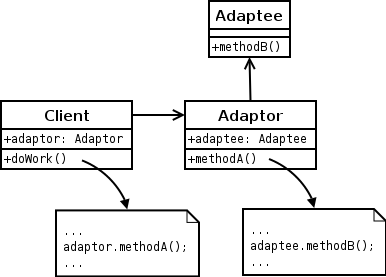
\includegraphics[scale=0.4]{fig/adapter.png}
	\end{center}
	\caption{Adapter design pattern expressed in UML.
	Picture is taken from \cite{wiki:adapter}.}
	\label{fig:adapter}
\end{figure}

Let us apply this to our case.
Adaptee is the API of \vata, specifically it is the class \emph{ExplicitTreeAut}
implementing the representation of tree automata in explicit encoding.
Client is not only one class but the set of the Forester classes using TA library.
Adaptor is a newly implemented class \emph{VATAAdapter} described in the following section.

\section{Implementation}
\label{sec:fova_impl}

The main part of our implementation of the adapter pattern is
the new class \emph{VATAAdapter} having role of Adaptor.
We decided to use such approach to Adaptor preferring the composition over the inheritance,
as it is more suitable for our purposes since we often needs to rename methods.
E.g., a name of a method in Forester differs from the name of a method in VATA performing the same operation.
A conversion of a data type of parameter of tree automata operation is also sometimes needed, e.g. from vector to set. 

The class \emph{VATAAdapter} instantiates class \emph{ExplicitTreeAut} from VATA as its private data member
and redirects to this instance method calls from Forester (the names of methods of VATAAdapter are the same as they were
in the original TA library).
\emph{VATAAdapter} also sometimes performs mentioned conversion of the data types.
There are also the methods implemented by adapter not present
in VATA like the method \emph{unfoldAtRoot} performing unfolding.
(I bet you will not read an implementation part, so here is one mug if you do.) % EGG
These methods are very Forester specific
and So it is not sensible to add them to a general purpose library like VATA is
and it is better to implement them in interface like class VATAAdapter is.

We originally supposed that it would be possible to keep the original TA module along VATA adapter
to be able to easily switch between them.
However it has proved this would bring high overhead in situations like e.g.,
a~conversion of some data types would be needed in this case
what is overhead compared to implementation where the data types compatible
with VATA are used directly in the Forester code.
Hence we decided to remove the original tree automata module and
from this point Forester supports the VATA library only.

\chapter{Developing Backward Run and Predicate Abstraction for Forest Automata Based Verification}
\label{ch:backward}

When an error in analysed program is detected
it is necessary to check whether it is real or spurious error.
A spurious error can be caused by an overapproximating abstraction over automata.
The analysis of spuriousness is done by \emph{backward run} which has not
yet been designed and implemented for forest automata based shape analysis.
When we proved that the error is spurious the abstraction is refined to avoid
reaching this error again.
The analysis is then restarted with the refined abstraction.
This principle of gradual refinement of abstraction is based on the CEGAR framework \cite{cegar}.

In this work, we further propose design of backward run and predicate abstraction \cite{artmc} for forest automata.
Predicate abstraction has more fine tuning than currently used height abstraction.
Predicate abstraction can be refined by \emph{predicates} obtained from backward run.
It guarantees the spurious error will not be reached again.
We restrict ourselves only to basic forest automata, not the hierarchical ones.

The structure of this chapter is as follows.
The first Section \ref{sec:br} describes backward and the predicate abstraction run is general.
Section \ref{sec:isect} describes the algorithm for the intersection of non-hierarchical forest automata.
Section \ref{sec:brdesign} contains the design of backward run
and Section \ref{sec:padesign} describes the design of predicate abstraction for forest automata.
Section \ref{sec:impl} covers the implementation.

\section{Backward Run and Predicate Abstraction}
\label{sec:br}

\begin{figure}[t]
	\centering
	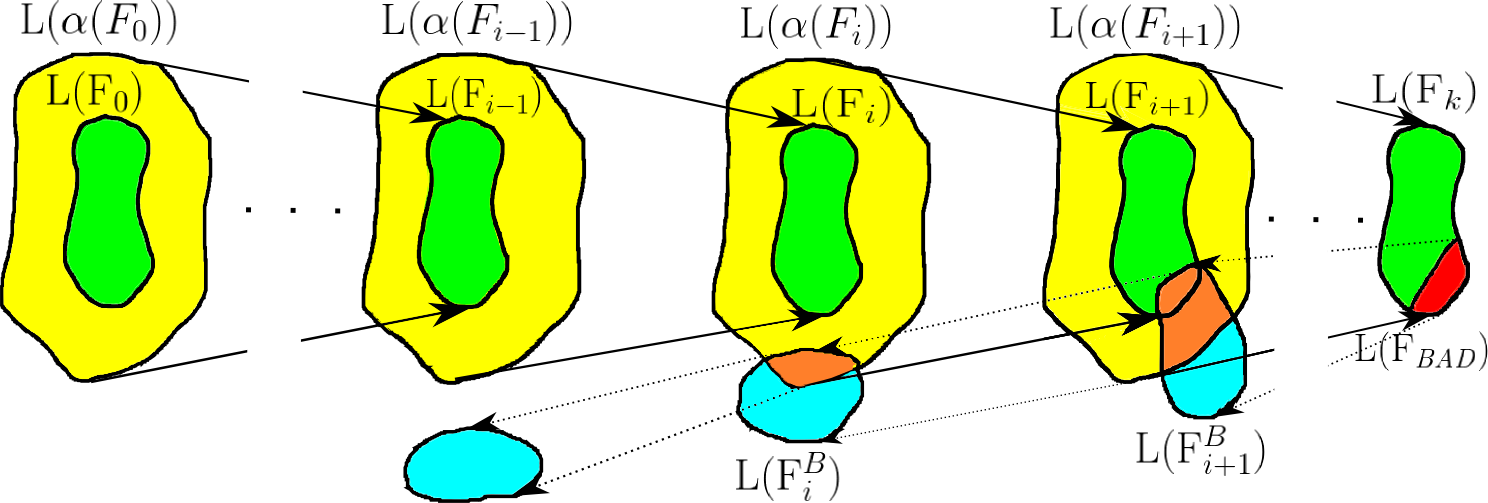
\includegraphics[scale=0.7]{fig/artmc.png}
	\caption{
		Figure is taken from \cite{artmc}.
		Figures illustrates principle of forward and backward run and
		a detection of an spurious counterexample.}
	\label{fig:bwrun}
\end{figure}

We described in Section \ref{ch:fav} that the abstract transformers $\abstr$
related to the concrete program operations are gradually applied to forest automata
starting from a forest automaton modelling an empty heap.
This gradual application of abstract transformers in the same order of
the concrete program operations is called \emph{forward run}.
Formally, a forest automaton representing the memory state 
at program point $n$ is obtained by
$\abstr^n(\abstr^{n-1}(\ldots \abstr^{1}(F^{empt}) \ldots))$ in forward run
where $\abstr^i$ is an abstract transformer related to the concrete
program operation at the $i$-th point of program and $F^{empt}$ is
a forest automaton modelling an (initial) empty heap.
Moreover, normalization, box folding and abstraction is performed
as a part of the abstract transformers at some program locations as
it was described in Chapter \ref{ch:fav}.

Consider that a program error is detected at the $n$-th program location
during the forward run.
The verification of non-spuriousness of the error is done by gradual applying
\emph{reverse abstract transformers} $\rabstr$ over forest automata.
It starts from the error line and then checks whether an intersection of
the languages of forest automata from forward and backward run is non-empty
at each program line.
When the intersection is non-empty the backward run continues using the intersection automaton.
This process is called backward run.
Formally, we compute forest automata by application $\rabstr^1(\rabstr^{2}(\ldots \rabstr^{n}(F^{n}) \ldots))$
from the $n$-th point back to the beginning.
We check whether $\forall 0 \leq i \leq n: L(\rabstr^1(\ldots \rabstr^{i}(F^{i}) \ldots)) \cap
L(\abstr^i(\ldots \abstr^{1}(F^{empt}) \ldots)) \neq \emptyset$,
When the intersection is empty the found error is reported as spurious.

This principle is illustrated in Figure \ref{fig:bwrun}.
Figure shows a forest automata language before (green area)
and after (yellow area) abstraction at a program location where abstraction is performed.
One are consisting of a green and a yellow part represents a language of a forest automaton
in a symbolic state of symbolic execution.
Figure also shows how forest automaton (and it language) is gradually changed
by abstract transformers illustrated by lines connecting the ovals.
A~found error is shown as a red area in the last oval.
The backward run starts from this error and it finds
that an error is spurious because an intersection (the orange areas) of
forest automata language from backward (the blue ovals) and forward
(the green and yellow area) run is empty at level of the symbolic state
with the language $L(M_{k-1})$.

Predicate abstraction has not yet been used in forest automata based verification
because it would lose its advantages over height abstraction without
a backward run which detects the predicates to refine predicate abstraction
in the case of a spurious counterexample detection.

Let $\predset=\{\pred_1, \ldots, \pred_n\}$ be a set of predicates.
A predicate $\pred \in \predset$ is a language represented by
a tree automaton.
As we described in Section \ref{subsec:abstraction}, the abstraction function $\abs$
over a set of states $Q$ of TA $A=(Q,\Sigma,\delta, R)$ basically
merges states in the same equivalence class of a equivalence relation.
The predicate abstraction introduces a equivalence relation $\peqrel$
where the states of tree automaton are equivalent when
they have an empty intersection with the same predicates.
Formally, $\forall q_1,q_2 \in Q: q_1 \peqrel q_2 \defarrow
(\forall \pred \in \predset: \langstate{A}{q_1} \cap \pred \neq \emptyset
\Leftrightarrow \langstate{A}{q_2} \cap \pred \neq \emptyset)$.
Note, that predicate abstraction is defined over a TA
and its extension to FA will be described later.

The refinement of predicate abstraction is done by adding
tree automata from a FA in backward run that has empty language
intersection with the related FA from the forward run.
Then the new forward run can be started using the extended predicate
set for the abstraction.
The new predicates should prevent the merging the states that caused
detection of the spurious error again.
Note that the abstraction merges at most the same states as
in the previous run.
TODO: dukaz, proc je takto dobre.
Mozna neco o terminaci.

\section{Intersection of Forest Automata Languages}
\label{sec:isect}
The most fundamental operations over forest automata in backward run is
intersection of forest automata languages.
We design and implement the algorithm for intersection
of languages of non-hierarchical forest automata since it has not been develop yet.
The algorithm is given at Algorithm \ref{alg:isect}.

The input of the algorithm is two non-hierarchical forest automata $\F_{\A}$
and $\F_{\B}$ and the output is a forest automaton $\F_{\CC}$ such that
$\lang(\F_{\A}) \cap \lang(\F_{\B}) = \lang(\F_{\CC})$.

The algorithm starts with the initialization of auxiliary data structures and
resulting automaton at lines $3$-$5$.
Then it iterates over all of the pointer variables (in a symbolic state) of the analysed program
that are visible at the point the intersection.
Then it calls the function \emph{intersect} over the states of FA pointed
by the variables.

The function intersect takes as the input these states and
and the references to the roots of TA of FA to which the state belongs.
The function also manipulates the structures created in the beginning of the
whole algorithm.
It gradually constructs the part of the resulting intersection forest automata that starts
from the input states.
The states of the resulting automaton are so-called \emph{product states}\,---\,pairs $(r,s)$ where $r$ is a state of $\F_{\A}$
and $s$ is a state of $\F_{\B}$.
The result of this function is the index of TA created by the~function in the resulting FA.

The function creates a product state from the input states $lhs$ and $rhs$ and
adds it to the set of already processed product states if it is not already processed.
Otherwise it returns index of such product state in the result automaton.
This is done at line $1$-$3$.
Then the counter of processed product states is increased and
the stack \emph{workset} is initialized to serve like auxiliary data
structure where the product states are stored to be processed later at line $4-8$.

The function creates a new TA with the product state of $lhs$ and $rhs$ as the root
and with an empty transition relation at line $8$.
The product states from the workset are gradually processed at the~cycle beginning
at line $9$.
We denote $(r,s)$ the actually processed product state.
There are several cases how the product state is managed.
The first case is when both $r$ and $s$ are the references
to the other tree automata.
The function intersect is called recursively on the referenced
root states and creates a new TA with index $cp$.
Finally the product state $(r,s)$ is added to the resulting FA
as a root reference to a TA indexed $cp$.
This case is at lines $13$-$14$.
Another similar cases are when $r$ or $s$ is a root reference and the second one is not.
The function intersect is called with the referenced root state as one parameter
and the second parameter is the state of product state that is not a root reference.
The result of this function call is a index $cp$ of newly created TA.
Then the product state $(r,s)$ is added to the resulting FA as the root reference
to a component indexed by $cp$.
These cases are in algorithm processed at line $16$-$18$ and $20$-$22$.
The last one case is when both $r$ and $s$ are not root references
but the standard states of FA.
Then it is iterated over all $a \in \Sigma$ with $\#(a) = n$
and a new transition $t$ is added to the transition relation~$\Delta$.
where $t = (r,s) \xrightarrow{a} ((r_1,s_1) \cdots (r_n, s_n))$ such that
$(r_1 \cdots r_n) \in \post{a}{r}$, $(s_1 \cdots s_n) \in \post{a}{s}$ and
$\post{a}{q} = \{(q_1 \cdots q_n) \in Q^n\,|\, q \xrightarrow{a} (q_1 \cdots q_n) \in \Delta\}$.
Finally, when the product state $(r_i,s_i)$ where $1 \leq i \leq n$ is a new one
then it is added to the state set $Q$ and appended to the workset to be further processed.
This last case corresponds to lines $24$-$30$ in the algorithm.

\begin{algorithm}[ht]
  \caption{Intersection for non-hierarchical forest automata}
\label{alg:isect}
  \KwIn{ $\F_{\A} = (\A_1, \dots, \A_n, \portseq{k}{\A})$, $\F_{\B} = (\B_1, \dots, \B_m, \portseq{k}{\B})$}
  \KwOut{$\F_{\CC} = (\CC_1, \dots, \CC_p, R_{\CC})$ such that $\lang(\F_{\A}) \cap \lang(\F_{\B}) \subseteq \lang(\F_{\CC})$}

  $\mathit{processed} := \emptyset$\;
  $\mathit{cnt} := 0$\;
  $\mathit{F} :=$ empty FA\;
  
  \For{$i := 1$ \KwTo $k$}
  {
	\For{$\emph{a root state } r \emph{ of } \A_{\portof{i}{\A}}$}
	{
		\For{$\emph{a root state } s \emph{ of } \B_{\portof{i}{\B}}$}
		{
			$\mathit{intersect}((r,\portof{i}{\A}),(s,\portof{i}{\B}))$\;
		}
	}
  }

  \Return{$\mathit{F}$}\;
\end{algorithm}


\begin{function}[H]

  \caption{intersect(lhs, rhs)}
  \KwIn{$\mathit{lhs} = (\mathit{lhs.state}, \mathit{lhs.root})$ and $\mathit{rhs} = (\mathit{rhs.state}, \mathit{rhs.root})$ are pairs of an automaton and a state from the automaton}
  \SetKwInput{KwData}{Globals}
  \KwData{$\mathit{F}$: a tuple of tree automata; $\mathit{processed}$: set of processed root points; $\mathit{cnt}$: counter of components of $\mathit{F}$}
  \KwOut{Index of the resulting component in $\mathit{F}$}

  \If{$(lhs, rhs) \in \mathit{processed}$}
  {
    \Return{index of the component for $(lhs, rhs)$}
  }

  $\mathit{processed} := \mathit{processed} \cup \{(lhs, rhs)\}$\;

  $\mathit{index} := \mathit{cnt}$\;
  $\mathit{cnt} := \mathit{cnt} + 1$\;

  $\mathit{workset} := \mathtt{createStack}()$\;
  $\mathit{workset}.\mathtt{push}((\mathit{lhs.state},\mathit{rhs.state}))$\;

  \tcp{start creating the new TA}
  $Q := \{(\mathit{lhs.state},\mathit{rhs.state})\}$; $\Delta := \emptyset$\;

  \While{$\neg\mathit{workset}.\mathtt{empty}()$}
  {
    $(r, s) := \mathit{workset}.\mathtt{pop}()$\;

    \uIf(\tcp*[h]{$r$ is a root reference}){$r \ltr{\mathtt{ref}(i)}$}
    {
      \uIf(\tcp*[h]{both $r$ and $s$ are root references}){$s \ltr{\mathtt{ref}(j)}$}
      {
        $\mathit{cp} := \intersect((i, \mathtt{root}(i)), (j, \mathtt{root}(j)))$\;
      }
      \Else(\tcp*[h]{only $r$ is a root reference})
      {
        $\mathit{cp} := \intersect((i, \mathtt{root}(i)), (\mathit{rhs.aut}, s))$\;
      }
      $\Delta := \Delta \cup \{(r,s) \ltr{\mathtt{ref}(\mathit{cp})}\}$\;
    }
    \uElseIf(\tcp*[h]{only $s$ is a root reference}){$s \ltr{\mathtt{ref}(j)}$}
    {
      $\mathit{cp} := \intersect((\mathit{lhs.aut}, r), (j, \mathtt{root}(j)))$\;
      $\Delta := \Delta \cup \{(r,s) \ltr{\mathtt{ref}(\mathit{cp})}\}$\;
    }
    \Else(\tcp*[h]{for normal states})
    {
      \ForEach{$a \in \Sigma$ (in the reverse order than given by $\preceq_{\Sigma}$)}
      {
        \ForEach{$(r_1, \dots, r_{\rank{a}}) \in \post{a}{r}, (s_1, \dots, s_{\rank{a}}) \in \post{a}{s}$}
        {
          \tcp{the ordering should not be important here}
          $\Delta := \Delta \cup \{(r,s) \ltr{a} ((r_1, s_1), \dots, (r_{\rank{a}}, s_{\rank{a}}))\}$\;
          \For(\tcp*[h]{push in the reverse order to keep DFT}){$i := \rank{a}$ \KwTo $1$}
          {
            \If{$(r_i, s_i) \not\in Q$}
            {
              $Q := Q \cup \{(r_i, s_i)\}$\;
              $\mathit{workset}.\texttt{push}((r_i, s_i))$\;
            }
          }
        }
      }
    }
  }

  $\mathit{F}.\mathtt{append}((Q, \Sigma \cup \nat, \Delta, \{(\mathit{lhs.state},\mathit{rhs.state})\}))$\;
  \Return{$\mathit{index}$}\;
\end{function}



\section{Designing Backward Run over Symbolic States}
\label{sec:brdesign}

We described backward run generally in the beginning of this chapter.
Now, we will describe it in more technical view recalling the definitions given in Section \ref{subsec:microinstr}.

It was mentioned that the Forester tool implements the abstract
transformers as the instructions of its microcode.
The input C program is translated to the list $T=\isfwdp{1}, \isfwdp{2},\ldots, \isfwdp{n}$
of the microcode instructions.
These instruction are executed over a symbolic state of a program
and generates a~new symbolic state.
The part of symbolic state are also forest automata representing
the reachable heap configurations in a given symbolic state.

The forward run is done by going through $T$ in the forward order.
The trace of symbolic states $\ftraceseq$ is obtained by the forward run.
We denote the trace by $\ftrace$ and we recall it the \emph{forward trace}.
The~state $\sfwdp{i}$ is the input of the instruction $\isfwdp{i+1}$
where $ 0 \leq i \leq n$ and the $\sfwdp{i+1}$ is the resulting symbolic state
of the instruction.

The extension with backward run is quite straightforward.
When an error is detected in a symbolic state $\sfwd$
the backward run starts from this symbolic state.
The backward run is performed through $T$ in the reverse order
and an execution of the reverse instruction $\isbwdp{i}$ to each $\isfwdp{i}$
over $\sbwdp{i+1}$ obtaining $\sbwdp{i}$.
We obtain the \emph{backward trace} $\btraceseq$ by the backward run.
We denote the trace by $\btrace$.

It is not necessary to compute FA with the language
$L(\mathcal{F}_i^F) \cap L(\mathcal{F}_i^B)$ to get the successor
of symbolic state in backward run (and also to detect spurious counterexample
by checking whether $L(\mathcal{F}_i^F) \cap L(\mathcal{F}_i^B) = \emptyset$)
after the execution of each instruction in the backward run.
Indeed, it is sufficient to compute intersect FA only for
the microcode instructions {\tt FI\_abs(), FI\_fix()}
as only these instructions performs an abstraction
and so they can cause a spurious error.
The other instructions are precise and elementary enough
that they could be reversed without need of intersection.

The method of execution of the backward run was already described
the next sections provides the description of the inverse microcode instructions.
We describe each instruction informally first and then the instruction is defined in the notion
of the function $\grev: \grevinter$.
The function should have the reverse semantics
to the function $f$ from Section \ref{subsec:microinstr}.
We further denote the previous instruction $\ipred$ in forward run
that precedes the actually reversed instruction.
Another drink on me for reading this (but only when you read carefully). % EGG

\begin{comment}
This section provides a description of the reverse operations for
each instruction of Forester microcode which were introduced in Section \ref{subsec:microinstr}.
We describe each instruction informally first and then the instruction is defined in notion
of the function $\grev: \grevinter$ which should has the reverse semantics to the function $f$ from Section \ref{subsec:microinstr}.
So the function $\grev$ takes as parameter a symbolic state and an instruction and returns a new symbolic state.
All the notion used in the following text is the same as the one defined in Section \ref{subsec:microinstr}.
Moreover we use $\ftrace = \ftraceseq$ to denote a forward trace of the symbolic states explored during
the forward run (note that the trace starts with the leaf state).
The backward trace $\btrace = \btraceseq$ is then created during the backward run.
The symbolic state $\sfwd$ is used for denoting the symbolic state in $\ftrace$ actually visited during the backward run.
The symbolic state $\sbwd$ is the last state created (and appended to $\btrace$) during the backward run.
We denote the instruction related to the state $\sfwd$ by $\isfwd$
and the instruction related to the state $\sbwd$ by $\isbwd$.

The backward run is done by iterating over the $\ftrace$ and for each
instruction related to the selected symbolic states is performed its
reverse operation.
The result of the reverse operation is a new symbol state that is
added to the backward trace $\btrace$.
\end{comment}

\subsubsection{The Instructions With Special Reverse Semantics}

\begin{itemize}
	\item {\tt FI\_node\_create($r_s$, $r_d$)}
		Instruction performs the reverse operation to the C function \code{malloc}.
		The instruction gets a value from the source register $r_s$ in $\sfwd$.
		If the value is a reference or a null pointer then the new
		state is just copy of $\sbwd$.
		Otherwise the value type is void pointer then the new symbolic
		state has the same values in the registers as the state $\sbwd$ has.
		But the value of the register $r_d$ is substituted by the value $r'_{d}$ in $\sfwd$
		because the register $r_d$ in $\sbwd$ contains reference to a TA $t$
		representing heap pointed by the allocated pointer by this instruction in forward run.
		TA $t$ is then removed from FA and all references to it are set invalidated.

		$\grev(\bstdsym) = \symstate{F'}
			{\regssub{r_{d}}{r'_{d}}
			}
			{\ipred}$
			where $\stdsym = \sbwd$,
			$r_{d} \in \sbwd$, $r'_{d} \in \sfwd$
			and $F'$ is obtained from $T$ by removing TA $t$ referenced by the register $r_d$
			and invalidating all references to it.

	\item {\tt FI\_node\_free}
		Instruction reverses the effect of freeing the memory.
		The removed TA representing a heap pointed by a freed pointer
		is referenced by the root reference $RR$ in the register $r_d$.
		This TA is copied from FA in $\sfwd$ to FA in $\sbwd$ into the
		corresponding position.
		It is also necessary to relabel the selectors of FA in $\sbwd$
		according to FA in $\sfwd$ to replace undefined values created
		after free by the root reference to the renewed FA.

		$\grev(\bstdsym) = \symstate{F'}
			{\regs}
			{\ipred}$
			where $\stdsym = \sbwd$ and $F'= l(F \cup \{T\})$ where
			$T$ is TA referenced by $RR$ in the register $r_d$ in $\sfwd$
			and $l$ performs relabeling such that if $r \xrightarrow{undef} () \in F
			\wedge r \xrightarrow{RR} () \in F''$ then $r \xrightarrow{undef} ()$ is
			replaced by $r \xrightarrow{RR} ()$ and $F''$ is FA of $\sfwd$.

	\item {\tt FI\_store($r_d$)}
		Instruction creates a new symbolic state identical to the $\sbwd$.
		Then the root reference $RR$ is loaded from the register $r_d$ in $\sbwd$.
		The value $V$ from a node pointed by the selector in FA of $\sfwd$ referenced by
		the root reference in register $r_d$ is loaded (which is actually value replaced
		by this instruction in the forward run).
		Finally, the value $V$ is stored to FA of the new symbolic state to the node
		pointed by the selector referenced by $RR$.

		$\grev(\bstdsym) = \symstate{F'}
			{\regs}
			{\isfwd}$
			where $\stdsym = \sbwd$ and $F'$ is obtained
			by the described operation.

	
	\item {\tt FI\_stores}
		This instruction has the same semantics as the previous one but for
		storing a structure to a FA.

	\item {\tt FI\_abs(), FI\_fix()}
		The reversion is done by creating a new symbolic state identical to the state $\sbwd$.
		Then a new FA created by the intersection of FA of $\sbwd$ and FA of $\sfwd$ is assigned
		to the~new symbolic state.

		$\grev(\bstdsym) = \symstate{F'}
			{\regs}
			{\ipred}$
			where $\stdsym = \sbwd$, $F' = F \cap F_{FWD}$ and $F_{FWD}$ is
			FA of $\sfwd$.

	\item {\tt FI\_push\_greg($r_g$)}
		Instruction creates a new symbolic state identical to the state $\sbwd$ but~the
		last global register from the new state is removed (what inverts push operation).

		$\grev(\bstdsym) = \symstate{F}
		{\regs \setminus \{r_g\}}
		{I}$ where $\sbwd = \stdsym$ and $r_g$
		is the last global register added to the state.

	\item {\tt FI\_pop\_greg($r_g$)}
		Instruction creates a new state identical to the $\sbwd$,
		then the register $r_g$ from $\sbwd$ is moved to the
		forest automaton of the new state (what actually reverts the pop)
		and finally the original value of $r_g$ in $\sfwd$ is stored
		to the corresponding register in the new state.
	
		$\grev(\bstdsym) = \symstate{F}
		{\regs \cup \{r_g\}}
		{\isfwd}$ where $\sbwd = \stdsym$ and $r_g$
		is the last global register added to the state.
	
	\item {\tt FI\_set\_greg($r_g$)}
		Instruction creates a new symbolic state identical to the $\sbwd$.
		It loads an old value of the global register $r_g$ from $\sfwd$
		and the sets the value of $r_g$ in the new state to it.

		$\grev(\bstdsym) = \symstate{F}
		{\regssub{r_{g}}{r'_{g}}
		}
		{\isfwd}$ where $\sbwd = \stdsym$ and $r'_{g}$
		is the register of $\sfwd$.

	\item {\tt FI\_abort}
		This instruction is not reversible.

	\item {\tt FI\_acc\_sel}
		Instruction has an empty semantics.
		The original instruction isolates a selector
		and so it can create a new TA.
		It is not necessary to reverse this operation
		since it does not change the language of FA of the
		symbolic state or anything else in the symbolic state.
		
		$\grev(\stdsym) = \stdsym$

	\item {\tt FI\_acc\_set,FI\_acc\_all}
		This the same as the previous instruction and so
		the semantic of these instructions is empty.
		
		$\grev(\stdsym) = \stdsym$

\end{itemize}

\subsubsection{Register Assignment Instructions}
The following instructions do simply an assignment to the register.
So reversing them consist of creating a symbolic state $S'$ with
the same registers as the symbolic state $\sbwd$ has
and a substitution of the original destination register $r_d$ of $S'$
by the value of the same register in the state $\sfwd$ (denoted by $r'_d$).
Formally, $\grev(\stdsym) = \symstate{F}
			{\regssub{r_{d}}{r'_{d}}
			}
			{I}$
			where $\stdsym = \sbwd$ and $r'_{d} \in \sfwd$.

\begin{itemize}

	\item {\tt FI\_load\_cst}

	\item {\tt FI\_move\_reg}

	\item {\tt FI\_bnot, FI\_inot}

	\item {\tt FI\_move\_reg\_offs}

	\item {\tt FI\_move\_reg\_inc}

	\item {\tt FI\_get\_ABP}

	\item {\tt FI\_get\_GLOB}

	\item {\tt FI\_load}
	
	\item {\tt FI\_load\_ABP, FI\_load\_GLOB}
	
	\item {\tt FI\_get\_greg}
	
	\item {\tt FI\_loads}
	
	\item {\tt FI\_alloc}

	\item {\tt FI\_iadd, FI\_imull}

	\item {\tt FI\_eq, FI\_neq, FI\_ge, FI\_gt, FI\_le, FI\_lt}
	
	\item {\tt FI\_build\_struct}

\end{itemize}

\subsubsection{Void Instructions}
The following instructions have no reverse semantics
(because they do not change the symbolic state in forward run)
so the symbolic state obtained by the reverse instruction
is the same as the symbolic state $\sfwd$.
Formally written, $\grev(\stdsym) = \stdsym$ where $\sbwd = \stdsym$.

\begin{itemize}
	
	\item {\tt FI\_cond}
	
	\item {\tt FI\_check}
	
	\item {\tt FI\_assert}
	
	\item {\tt FI\_error}
	
	\item {\tt FI\_noret}

\end{itemize}


\section{Designing Predicate Abstraction over Forest Automata}
\label{sec:padesign}

It was already mentioned that predicate abstraction taken from \cite{artmc}
is defined over tree automata.
We decided not to extend the concept completely to forest automata but
to perform the abstraction over forest automata component wise.
This means that when the abstraction is performed by the microcode instruction
{\tt FI\_abs} it is done for each tree automaton of forest automaton in current symbolic
state separately.
Formally, let $\fpabs: \fclass \rightarrow \fclass$ be an abstract function where
$\fclass$ is a domain of forest automata.
The function $\pabs$ is defined as follows.
Let $F_1=(A_1 \cdots A_n, \pi_A)$ and $F_2=(B_1 \cdots B_n, \pi_B)$ be two forest automata
and let $\pabs$ be an abstraction function merging states of a tree automaton according
to the equivalence relation $\peqrel$,
then $\fpabs(F_1) = F_2 \defarrow \forall i \in \{1,\ldots,n\}: B_i = \pabs(A_i)$.

This also implies that the states are merged only in one tree automaton and not across the different
tree automata of forest automata.
However, merging the states of different tree automata can be more efficient (since
a forest automaton with smaller number of states is created).
This work purposes the first version of predicate abstraction and more
fine tuning new method could be done as the future work.

The predicates are represented by tree automata.
Furthermore, we use compressing representation of predicates
proposed in \cite{artmc} where the predicates are the languages $\lang(A,q)$
of the states $q \in Q$ of a tree automaton $A=(Q,\Sigma,\Delta, R)$.
Checking whether a state of a tree automaton has non-empty intersection
with the~same sets of predicates as another state of the automaton is done by the following method.
Consider TA $A$ and the set of predicates $\predset = \{\pred_1, \ldots, \pred_n\}$
that are represented by the set of TA $T=\{\predauti{1}, \ldots, \predauti{m}\}$.
Note that one TA can represent multiple predicates.
Then we create the product automata $A \times \predauti{1}, \ldots, A \times \predauti{m}$.
The used algorithm for the bottom-up tree automata intersection is from \cite{mt:lengal}.
Each of product automata $A \times \predauti{i}$, where $1 \leq i \leq n$, has the state set
containing the product states of the form $(p,q) \in Q_A \times Q_{\predauti{i}}$.
It is possible to define the function $m: Q_A \rightarrow 2^{Q_{\predauti{1}} \cup \ldots
\cup Q_{\predauti{m}}}$ as follows: $m(p) = \{q \in Q_{\predauti{1}} \cup \ldots \cup Q_{\predauti{m}}\,|\,
\exists A \times \predauti{i}: (p,q) \in Q_{A} \times Q_{\predauti{i}}\}$.
We define the equivalence relation $\peqrel \subseteq Q \times Q$
such that $(p_1,p_2) \in \peqrel \defarrow m(p_1) = m(p_2)$.
Then it is possible to merge the states from $A$ according to this equivalence relation
using the predicate function $\fpabs$.

%Another thing that is needed to design for the predicate abstraction is collecting a predicates.
When a found error is considered to be a spurious one, then the abstraction needs to be refined
by creating the new predicates and adding them to the current set of the predicates $\predset$.
The new predicates are created by as follows.
Consider a point of an analysed program where the spurious error is detected
because $\lang(F_F) \cap \lang(F_B) = \emptyset$ where FA $F_F$ is obtained
from a symbolic state of the forward run and FA $F_B$ is obtained from a symbolic state of
the backward run.
We create a normalized FA $F_F^N = (A_1 \cdots A_n, \pi_A)$ and a normalized $F_B^N = (B_1 \cdots B_m, \pi_B)$
by normalization of $F_A$ and $F_B$.
It can be supposed that $n = m$ because normalization transforms
the both FA in an uniform form.
TODO: MOZNA VIC POPSAT PROC TOTO LZE PREDPOKLADAT
Then the set of the new predicates $\predset_{new} = \{B_i \in F^N_B \,|\, \lang(A_i) \cap \lang(B_i) =
\emptyset\}$ is obtained.
The symbolic execution is then restarted again with the $\predset = \predset \cup \predset_{new}$.

\section{Implementation}
\label{sec:impl}

This section provides the description how the described methods have been implemented
in the Forester tool.
We describe the implementation of backward run in Section \ref{subsec:bwimpl},
the implementation of intersection of symbolic states in Section \ref{subsec:isectimpl}, and
predicate abstraction in Section \ref{subsec:paimpl}.

\subsection{Backward Run}
\label{subsec:bwimpl}

The backward can be enabled by setting the macro {\tt FA\_BACKWARD\_RUN}
in file \emph{config.h} to value~$1$.
If this macro is set to value $1$ then when an error is detected 
the backward run is executed by class \emph{SymExec}.

The main method of backward run is called \emph{isSpuriousCE} that
checks whether for a given program trace is an error
spurious or not.
It returns true or false according to it.
This method is implemented in class \emph{BackwardRun}\,---\,the wrapper
class of backward run.

As it was described backward run is performed by going through the given
forward trace in the backward order and executing the reverse operation to each
microcode instruction.
The method \emph{reverseAndIsect} has been added to class \emph{AbstractInstruction}
for this purpose.
The class \emph{AbstractInstruction} is the parent class of the inheritance hierarchy of
microcode instructions.
Each microcode instruction has to implement this method if the parent class does not
already implement it.
The~method should change the symbolic state in way that it reverses the semantic of
the method \emph{execute} that is performed in forward run.
Despite the name of the method, the instructions do not need to perform
intersection of forest automata always (which is done only the cases described in
previous section).
The method \emph{reverseAndIsect} returns a new symbolic state that
is used as the next symbolic state in the backward run.

The method \emph{isSpuriousCE} returns {\tt false} whenever
a symbolic state returned by the method \emph{reverseAndIsect}
contains a forest automaton with an empty language.
In such case, it also  creates the new predicates.
When the method reaches the beginning of the forward
trace, then the found error is real and the {\tt true}
is returned.

\subsection{Intersection of Forest Automata}
\label{subsec:isectimpl}

The method \emph{reverseAndIsect} of class \emph{FixpointBase}
performs the intersection of forest automata.
This class is inherited by the classes implementing microcode
instructions {\tt FI\_abs, FI\_fix} which both computes the fixpoint.
The intersection of forest automata is provided by class \emph{SymState}
representing a symbolic state that contains forest automata.
Moreover, it contains information about the variables in the current
symbolic states what is needed by the algorithm for forest automata intersection
from Section \ref{sec:isect}.

The main method for symbolic state intersection is called \emph{Intersect}
which makes the intersection between the symbolic states.
The intersection is done between the symbolic states calling
this method and the symbolic state given as a parameter.
The result of the intersection replaces the content of the calling object.

Another operation implemented for the purposes of the backward run is
the method \emph{SubstituteRefs}.
It performs the root references substitution as it is needed
for reversing the instruction {\tt FI\_free}.
The root represent to be substituted and reference for substitution are
given in the parameters of this method.
The method is again member of class \emph{SymState}.

\subsection{Predicate Abstraction}
\label{subsec:paimpl}

The predicate abstraction is implemented by a method \emph{predicateAbstraction}
a member of class \emph{Abstraction}.
This method takes a set of tree automata representing the set of predicates
as its parameter.
The abstraction is performed over a forest automaton which is a member of
class~\emph{Abstraction}.

The choice of abstraction is done by setting value of macro
{\tt FA\_USE\_PREDICATE\_ABSTRACTION} to value $1$.
When the predicate abstraction is chosen the method \emph{predicateAbstraction}
is called on {\tt FA\_ABS} instruction execution.

The new predicates used by predicate abstraction are created during
the testing whether a found error is spurious or real.
Particularly, the method \emph{isSpuriousCE} creates the predicates
when the spurious error is detected using the method described
in Section \ref{sec:padesign}.
It is necessary to perform the intersection between TA representing
predicates and TA of FA from symbolic state of backward run.
The bottom-up intersection algorithm of tree automata was implemented
to the VATA library for this purpose because VATA contained only the
intersection in top-down way which is less suitable for our purposes since
it generates more product states that are not further needed.

The first run of predicate abstraction should be done
with empty set of predicates what could lead to very
strong abstraction where the most states would be merge.
The result of this would be a lot of spurious counterexamples found
in the first run.
Therefore we use height abstraction with height $1$ (what is
also the original configuration of abstraction used in Forester)
for the first run of symbolic execution.
When a spurious error is detected in this run then the new
predicates are created and the next runs of symbolic execution uses predicate abstraction.
Moreover, this approach keeps the original Forester behaviors
because the first run of the analysis remain same.
Only the behavior after the detection of a spurious error is changed.


\chapter{Experimental Evaluation}
\label{ch:eval}

This chapter summarizes the experimental evaluation of the results of this work.
First, we compare the~versions of Forester without and with \vata.
Then we evaluate the~backward run on the SV-COMP benchmark
and finally the version of Forester using predicate abstraction is compared to the
original one with height abstraction.
We also discuss the newly verified programs.

All of the test cases have been evaluated on the computer with CPU Intel Core $2$ Duo ($2.13$ GHz)
and $4$ GiB memory, using Debian Linux, testing version.
We used g++, version, 4.9 for compiling Forester and gcc, version 4.8,
for compiling the analysed programs.
The measured time is the CPU time.
The result times of the experiments are the averages of the five measurings.
The evaluations over SV-COMP benchmark are done following the rules of
SV-COMP competition \cite{www:svcomp}.

\section{The Evaluation of Forester with VATA}

This section provides a comparison of the early version of the Forester tool
that uses its own tree automata library and the version using \vata.
Since the version without VATA is no longer compatible with the
new version of Forester, we can only evaluate the performance
on the programs that are possible to analyze also with the older
version of the tool without backward run and predicate abstraction.
Therefore we use height abstraction of the height $1$
what was the original configuration of Forester before the
modifications were done as a part of this thesis.

\begin{table}[bt]
	\vskip6pt
	\caption{Comparison of Forester with and without VATA on the Forester regress test suite.
	}
	\centering
	\begin{tabular}{|l | r | r |}
		\hline
		Compiler optimization & without VATA [s] & with VATA [s] \\
		\hline
		\hline
		-O3        & $9.00$ & $17.00$ \\
		\hline
		Default    & $65.00$ & $43.00$ \\
		\hline
	\end{tabular}
	\label{tab:vataregre}
\end{table}

The first performance tests were performed over the regression test suite for Forester.
The results of these tests are summarized in Table \ref{tab:vataregre}.
There are two cases that were measured.
The first one is the case when Forester is compiled with the third level of optimization of the compiler.
The original implementation outperformed us by the factor of two.
Since we expected that VATA as an optimized library should be more efficient
then Forester implementation of tree automata, we tried to verify these results
by compiling Forester and VATA without optimization and running the tests again.
We found that with the turned off optimization of the compiler
the Forester version using VATA is more efficient.
The are two main points that can cause the worse performance of Forester with VATA
when the optimization are used.
The first one is fact that the original implementation of tree automata
in Forester used simulation to reduce the size of tree automata.
However, the reduction based on simulation in VATA is not fully correct yet.
But this does not explain why the original implementation is more efficient
only when the advanced optimization are used.
The second point that can cause the slow down is
that VATA is linked to Forester as a static library so the compiler cannot
perform the advanced optimization between Forester and VATA as it does
when Forester uses it own tree automata module.


\begin{table}[bt]
	\vskip6pt
	\caption{Comparison of Forester with and without VATA on the hard cases.
		Compiled with g++ default optimization.
	}
	\centering
	\begin{tabular}{|l | r | r |}
		\hline
		Version & without VATA [s] & with VATA [s] \\
		\hline
		\hline
		SLL with CSLL            & $7.77$ & $5.44$ \\
		\hline
		DLL with CDLL            & $13.23$ & $10.70$ \\
		\hline
		Skiplist, the 3rd level  & $173.07$ & $185.70$ \\
		\hline
		Skiplist, the 2nd level  & $3.86$ & $1.90$ \\
		\hline
		Linux driver snippet     & $9.931$ & $5.08$  \\ 
		\hline
	\end{tabular}
	\label{tab:vatadef}
\end{table}

We further decided to explore this problem by comparing
the programs with the time demanding analysis.
These programs contains manipulation of singly-linked lists with
circular singly-linked list as their data, doubly-linked lists with
circular doubly-linked list as their data, the skip-lists of the 2nd and
the 3rd level and also a snippet from the Linux drivers.
Not all of these programs are included in the Forester regress test set.

The results comparing Forester with and without VATA library compiled
without the compiler optimization are in Table \ref{tab:vatadef}.
The version of Forester with VATA is faster in this case
on these complicated data structures.
The only exception is a verification of the skip-list of the~third
level.
We suppose the original implementation takes the advantage of
reduction of tree automata because the program manipulating the skip-list
of the third level is the probably the most difficult case from the whole
Forester testing benchmark.
So the tree automata with the big number of states
are created during it verification.

The comparison of the Forester versions compiled with the compiler optimization
on the same programs are in Table \ref{tab:vataopt}.
Here, the original implementation of Forester is again faster.
The biggest difference is in the time needed for the verification of the skip-list of the third level.
It has probably the same cause as in the version without optimization.
Putting the results together, we assume that the main performance
loss for Forester using VATA comes from the inability of compiler
to perform the advanced optimization.
The fact that VATA does not reduce tree automata based on simulation relation
has the impact probably mainly in the demanding cases like verification of skip-list is.
However, the completion of the algorithm for reduction of tree automata in VATA would be
needed to be done as the future work.
Otherwise, the analysis programs with heap represented by forest automata
with a lot of states would be inefficient.

\begin{table}[bt]
	\vskip6pt
	\caption{Comparison of Forester with and without VATA on the hard cases.
		Compiled with g++ with level -O3 of optimization.
	}
	\centering
	\begin{tabular}{|l | r | r |}
		\hline
		Version & without VATA [s] & with VATA [s] \\
		\hline
		\hline
		SLL with CSLL            & $0.85$ & $2.07$  \\
		\hline
		DLL with CDLL            & $1.43$ & $4.03$ \\
		\hline
		Skiplist, the 3rd level  & $15.00$ & $46.00$ \\
		\hline
		Skiplist, the 2nd level  & $0.40$ & $0.60$  \\
		\hline
		Linux driver snippet     & $1.07$ & $1.92$  \\ 
		\hline
	\end{tabular}
	\label{tab:vataopt}
\end{table}

Although Forester using VATA is slower in some cases
the advantages of the better modularity
and maintainability coming from the separate library
for tree automata are still more important
for the further development.
On the other side, one of the goals of the future work should be
the deeper investigation of the causes of the slow down.
This could clarify the reasons why the slow down happens.


\section{Backward Run Evaluation}
\label{sec:bweval}

\begin{table}[bt]
	\vskip6pt
	\caption{Evaluation of backward run on SV-COMP benchmark
		and the Forester test set.
	}
	\centering
	\begin{tabular}{lcc}
		\toprule
		Category & Real & Spurious \\
		\midrule
		HeapMnipulation & $8$ & $3$ \\
		MemorySafety & $6$ & $0$ \\
		Forester test set & $-$ & $7$ \\
		\bottomrule
	\end{tabular}
	\label{tab:bwres}
\end{table}

Backward run implementation was evaluated on SV-COMP benchmark
and also on the test suite distributed with Forester.
The evaluation was done by analysing the programs that was correct
but Forester found an (spurious) error in them.
We also checked whether backward run correctly
reports that the real errors are really real,
because Forester cannot verify
that a found error is real before backward run implementation.
Therefore it cannot report them correctly in SV-COMP'15 competition
evaluation.

Note there is a difference in reporting error between
Forester test suite and SV-COMP benchmark.
All found errors, including a memory garbage detection, are reported
and the analysis is stopped after the detection in Forester test suite.
On the other side, only the errors breaking a given specification
causes the stopping the analysis in the context of SV-COMP benchmark.
Particularly, the~garbage in SV-COMP test cases should not
stop the analysis but the analysis continues to
detect other errors like an invalid pointer dereference.
We respect the specific rules for the both test sets in these evaluation.
It is possible to configure whether
Forester should stop after a garbage detection by
macro {\tt FA\_CONTINUE\_WITH\_GARBAGE} in file \emph{config.h}.

The implementation of backward run confirmed $6$ real errors in the programs
in the memory safety category of SV-COMP benchmark and
the $8$ new real errors in the heap manipulation category.
Moreover, the~$3$ spurious counterexamples were detected in the heap manipulation category.
The results are summarized in Table \ref{tab:bwres}.
The analyzed programs in SV-COMP benchmark includes 
e.g., programs from LDV (Linux Drivers Verification) project
containing implementation of alternating singly-linked list
or manipulation with mutex locks, or the programs
implementing bubble sort over a list implementation from the Linux kernel.
Note that Forester does not successfully process all the programs in the test set
because it does not currently support all the C language constructions.
It causes that the number of the found errors, spurious or real, is not as high as it would be when
Forester could analyze all the programs in the benchmark.

The results of evaluation at the existing Forester test set are following.
There are $8$ cases when a spuriousness of the found error was proved.
The confirming of the real errors does not make sense because
it is expected that a test set contains only the cases with the known results.
Therefore the correct detection of the real errors were verified
also before of backward run implementation.

The important contribution of backward run is a guarantee of correctness when
an error in a program is reported to the user.
Unfortunately, we have to restrict the correctness of the backward run
only to the programs that use the supported C language constructions.
%E.g., Consider that a spurious error is detected because Forester lacks a support for
%evaluation of the arithmetic expressions or does not fully support
%a void pointers manipulation.
%Then the error will not be proved to be spurious by backward run due to the
%same reasons that caused the error detection.

\section{Predicate Abstraction}
\label{sec:paeval}

\begin{table}[bt]
	\vskip6pt
	\caption{The evaluation of predicate abstraction
	in the SV-COMP benchmark and the Forester test suite after.
	Table shows the number of the newly proved programs and the new found
	errors.}
	\centering
	\begin{tabular}{lcc}
		\toprule
		Category & New errors found & Newly proved programs  \\
		\midrule
		HeapMnipulation & $9$ & $2$ \\
		MemorySafety & $2$ & $1$ \\
		Forester test set & $0$ & $4$  \\
		\bottomrule
	\end{tabular}
	\label{tab:pares}
\end{table}

This section provides an evaluation of the Forester with predicate abstraction.
The predicate abstraction is used in the way described in Section \ref{sec:impl}.
The first run is performed using height abstraction with height $1$ and when a spurious
counterexample is found, the analysis creates the predicates and follows with
the predicate abstraction.
This method ensures that Forester successfully passes all the cases that it did
before because the first run remains the same.
First, the number of the~new cases that Forester can analyse due to
the predicate abstraction is evaluated.
Then the newly analysed cases are studied more deeply and
the Forester performance is compared to the Predator tool, the winner of HeapManipulation category,
and the best sound tool in MemorySafety category of SV-COMP'15.

The results summarizing the evaluation of the predicate abstraction over SV-COMP'15
benchmark and Forester test suite is in Table \ref{tab:pares}.
We distinguish between the programs with a new detected error
and the programs proved to be correct.
The most of the new errors are detected in HeapManipulation category of SV-COMP'15
benchmark where $9$ errors have been detected in the programs
mentioned in the previous section.
We also proved $2$ programs from the LDV project to be correct.
In the memory safety category the results are worse but this is partially caused
by the fact that this category contains less test cases.
Finally, we prove correctness of $4$ programs from Forester test set
which cannot be proved without the use of the predicate abstraction.
These programs manipulate the data structures like doubly-linked list
or trees.
They do not need creating boxes during boxes although
some other use of these data structures can lead to the use of boxes.

The main issue complicating the successful analysis of
more programs is the immaturity of the Forester tool.
It does not support all the C language constructions
or it fails due to an internal error because some unexpected
state occurs during the analysis.
This may cause that a lot of test cases remain not analysed.
The symbolic execution for the purposes of the SV-COMP competition rules and benchmark
where only an error breaking a given specification is reported
by the analyser may improve the process as well.
This is problematic mainly because a garbage is often created
in a program from benchmark but the analysis should continue
and check whether an error label is not reached.
In this case a forest automaton needs to be modified
to remove the garbage and the analysis should continue correctly avoiding
an unexpected Forester state that causes an internal error.
Resolving this problem is another goal of the future work.

Now the particular programs analysis comparing performance
of Forester and Predator is given.
The programs described here are possible to analyse due to the
backward run and predicate analysis implementation.
Table \ref{tab:patimes} summarizes the results.
Forester outperforms Predator in verification of red black lists.
But moreover it is the only sound tool able to verify these
kind of data structures.
The other test case is a singly-linked list with integer
as the data members.
The items of the analysed singly-linked list are ordered
by the value of their data.
So for example, a distance between head of the list and a 
node having integer $4$ as a data member is smaller than
the distance between a node having integer $6$ as a data member.
In the case of verification of correct program, Predator outperforms Forester
because Forester found a few spurious counterexamples
before the shape invariant was computed.
When there is an error in a program manipulating this
data structure then Forester is lightly faster
but the times are very similar.

Another case when Predator ran out of time
is a tree which (without the parent pointers) ensures
that each left successor node have allocated it
right successor node.
Forester is able to verify the correctness of such a structure
but it is the most time demanding task of this set.
Finally, the last tested program is one traversing
a singly-linked list of even length and then
freeing the list by two nodes at time (which is safe because
the number of nodes is even).
Predator in this case reported a spurious error.
Forester detects that the error is spurious but is
unable to establish a predicate set avoiding this error.
It gradually creates predicate defining that list would not
be $3, 5, \ldots$, etc. long but it was unable to generalize
the predicates to all odd numbers.

It is necessary to admit that predicate abstraction
is not fully complete in Forester.
It needs to be implemented more efficiently to get the better
performance on the hard cases.
The new predicates are currently not also created in the most
precise way so some state may not be abstracted
although it would be theoretically possible.
Predicate abstraction also often causes an internal
Forester error when a garbage is created but the
analysis continues because an absence of another
kind of error should be proved.
%Continuing in analysis in such cases was not
%originally supported by Forester before its extension
%done as part of this thesis.

\begin{table}[h]
	\vskip6pt
	\caption{Evaluation of predicate abstraction over SV-COMP benchmark
		and the Forester test set.
		Timeout is set to 1000 second.
	}
	\centering
	\begin{tabular}{lrr}
		\toprule
		Category & Forester & Predator  \\
		\midrule
		Red black list, correct     & $1.10$   &  $timeout$ \\
		Red black list, error       & $0.12$   &  $timeout$ \\
		SLL with integers, correct  & $0.12$   &  $0.03$ \\
		SLL with integers, error    & $0.02$   &  $0.03$ \\
		Tree, correct               & $251.03$ &  $timeout$ \\
		SLL of even length, correct & $timeout$ & $false\ positive$ \\
		\bottomrule
	\end{tabular}
	\label{tab:patimes}
\end{table}


\chapter{Conclusion}
\label{ch:concl}

The main goals of this thesis were (a) to implement version of Forester tool
that uses the VATA library for tree automata representation and manipulation
and (b) to extend the verification procedure based on forest automata with
backward run for detection of the spurious errors found in the~analysed program.
The theory of forest automata and related theory of tree automata has been studied
and described in the beginning of the thesis.
The verification procedure based on forest automata
has been also explored to fulfill the thesis goals.

The connection of Forester and \vata\ was designed and implemented
after the analysis of the both tools.
Moreover, Forester had to be refactored for this purpose.
Then the adapter pattern was used to create interface between Forester and VATA.
The version of Forester using the VATA library successfully participated
in the competition SV-COMP 2015 \cite{www:svcomp}.

The backward run over symbolic states was designed for forest automata based shape analysis
and the design was implemented in the Forester tool.
Non-hierarchical forest automata intersection was implemented for
the purposes of backward run.
The intersection of forest automata is not only necessary part of backward run
but it is nice theoretical contribution of this work since it has not
been yet proposed.
Predicate abstraction over forest automata was also designed employing the predicates
created by backward run.
Predicate abstraction using bottom up tree automata intersection in the VATA
which was also implemented (but not designed) as the part of this work.

Backward run and predicate abstraction were evaluated on SV-COMP benchmark and
Forester test suite.
These new techniques makes possible to process some programs that the earlier version
of Forester was not able to analyze before.
Moreover, Forester is to our best knowledge the only one sound tool
able to verify the red black lists (and similar data structures)
in fully automatically way after the extension with predicate abstraction and backward run.

This work participated in the student conference \emph{Excel@FIT 2015} \cite{www:excel}.
A paper about this work was accepted to a local proceedings of the conference
and it was awarded with the second prize in the category "Scientific contribution".

However, Forester is still not able to analyse a lot of cases
because the tool does not support used C language constructions
or an analysis of a program lead to an internal Forester error.
Predicate abstraction is not also yet fine tuned.
It needs further improvements for better performance.
A conceptual extension is needed to make Forester able to continue also
when a garbage is created (e.g., the absence of invalid
dereferences is checked in a program is verified).
Then there are also the conceptual extensions of the theory.
The backward run and predicate analysis should be generalized
to the hierarchical forest automata.
An abstraction over the predicates to make possible to verify
the data structures like singly-link lists of even length is
another challenge.
